\chapter{Continuous contrast variation in SAXS: the density gradient technique}
\label{chap:density_gradient_SAXS}
The contrast variation method in Small Angle X-ray Scattering (SAXS) experiments consists in systematically varying the electron density of the dispersing media to study the different contributions to the scattering intensity in greater detail as compared to measurements at a single contrast, as described in chapter \ref{chap:theory_SAXS}. It emerges as an ideally suited technique to elucidate the structure of particles with a complicated inner composition and has been repeatedly employed to investigate the radial structure of nanoparticles in suspension, e.g. latex particles suspended in an aqueous medium \citep{dingenouts_analysis_1999,ballauff_analysis_2011}. In Small Angle Neutron Scattering (SANS) the contrast variation technique is widely used by mixing water and deuterium oxide, but the use of deuterated chemicals and the incoherent contribution to the background as well as the limited access to neutrons restrict the application of this technique. Other methods for structural investigation (e.g. transmission electron microscopy \citep{joensson_morphology_1991,silverstein_microstructure_1989}) require prior treatment of the sample and are not ensemble averaged. 

In SAXS, the solvent contrast variation technique is achieved by adding a suitable contrast agent to the suspending medium (e.g. sucrose) and recording the scattering data as a function of the adjusted solvent electron density \( \rho_{\text{solv}} \) \citep{ballauff_saxs_2001-1,bolze_application_2003}. In order to resolve small changes of the radial structure, the average electron density of the colloidal particles must be close to the dispersant's, i.e., the \emph{match point} should be approached, where the average contrast of the particle vanishes. In the case of polymeric latexes with electron densities ranging from 335 to \(390 \mbox{ nm}^{-3}\), an aqueous sucrose solution is very well suited as the suspension medium, due to the easy realization of concentrated solutions with electron densities of up to \(400 \mbox{ nm}^{-3}\). Previous studies on globular solutes \citep{kawaguchi_isoscattering_1992} and the influence of the sucrose on the size distribution of vesicles \citep{kiselev_sucrose_2001-2} show the feasibility of this technique, while further studies have investigated the effect of the penetration of the solvent into the particles \citep{kawaguchi_isoscattering_1993}.

The preparation of a number of different sucrose solutions has been a major inconvenience in solvent contrast variation experiments, due to the tedious, time-consuming process, possible inaccuracy in the sucrose concentration and the discrete range of available solvent electron densities. In this chapter, a novel approach using a density gradient column is introduced, which allows the tuning of the solvent contrast within the provided density range, resulting in a virtually continuous solvent contrast variation. By filling the bottom part of the capillary with a particle dispersion in a concentrated sucrose solution and the top part with an aqueous solution of the same particle concentration, a solvent density gradient is initiated with a constant concentration of nanoparticles along the capillary. Density gradient columns are extensively used in fields like marine biology \citep{coombs_density-gradient_1981} or biochemistry together with centrifugation \citep{hinton_density_1978}, to create a continuously graded aqueous sucrose solution by diffusion of the sucrose molecules. By measuring the density gradient column at different points in time during the diffusion process of the sucrose, it is possible to choose \emph{in situ} the most appropriate solvent densities to perform measurements close to the contrast match point. Combining this approach with SAXS, a very extensive dataset with a virtually continuous variation in the suspending medium density can be acquired in a short interval of time.

The experimental details of the proposed approach are shown in section \ref{sec:DensityGradientExperimental}, followed by the example of the continuous contrast variation technique applied to polymeric nanoparticles in section \ref{sec:KiskerResults}. The evaluation of the SAXS data using different methods is reviewed in section \ref{sec:KiskerResultsEvaluation}, jointly with the discussion of the experimental measurements and a summary of the obtained results. Finally in section \ref{sec:applicability} the applicability of the solvent contrast variation technique in SAXS is discussed and compared to other contrast variation techniques.

\section{Experimental procedure}
\label{sec:DensityGradientExperimental}
Firstly, the preparation of a nanoparticle suspension density gradient within a glass capillary using an aqueous sucrose solution is described in section \ref{sec:GradientPreparation}. Then in section \ref{sec:SolventCalibration}, the calibration of the solvent electron density through X-ray transmittance measurements at different positions along the capillary vertical axis is explained, followed by a detailed overview in section \ref{sec:DensityGradientSAXS} of the collection of scattering patterns at the calibrated capillary positions with distinct contrasts.


\subsection{Preparation of the density gradient capillaries}
\label{sec:GradientPreparation}
The solvent density gradient is prepared in the rectangular glass capillaries presented in section \ref{sec:sample_environment}, which are extraordinary homogeneous and show very uniform sample thickness within 0.9 $\%$ and glass thickness within 0.4 $\%$. The bottom end of the capillary is closed by welding and the lower section, up to a height of ca. \(1\) cm, is filled with Galden\textregistered\ PFPE SV90 from Solvay Plastics (Brussels, Belgium). This fluid has an exceptionally high density of 1.69 g cm$^{-3}$, low viscosity and is immiscible with aqueous solutions. Consequently, a uniform interface with the particle suspension is formed at the bottom, which is employed as reference position for the X-ray transmittance measurements. 

The studied nanoparticles in suspension are mixed with a high sucrose concentration (Sigma-Aldrich, Missouri, USA) and diluted in an aqueous solution, creating two mixtures with different solvent densities but equal particle concentrations. Directly above the Galden fluid, the denser of these two mixtures is filled into the capillary using a syringe up to a height of about 1 cm. The lighter aqueous dilution is then filled on top of the aqueous sucrose solution along ca. 1 cm. By the time the two components come into contact, the density gradient is initiated and the sucrose starts diffusing along the ca. 20 mm length of the filled capillary.

The calculated diffusion timescale of the solvent density gradient is ca. 10 minutes, considering that the diffusion coefficient of sucrose in water at 25 $^{\circ}$C is $D=5.2 \cdot 10^{-10} \;\mbox{m}^2\,\mbox{s}^{-1}$ \citep{uedaira_sugar-water_1985,ribeiro_binary_2006} and assuming that convection effects are negligible due to the small length-scale of the capillary \citep{berberan-santos_barometric_1997}. The time needed for the transfer of the sample into the UHV sample chamber amounts to ca. 1 hour. Within this time duration, the deviation of the solvent density at both ends of the gradient from the initial value can be estimated with an uncertainty below 0.5 $\%$. 


\subsection{Calibration of the solvent density: X-ray transmission}
\label{sec:SolventCalibration}
The rectangular capillary is placed in the sample holder inside the UHV reflectometer described in section \ref{sec:fcm} which allows the movement with micrometer precision in the directions perpendicular to the incoming beam, as depicted in figure \ref{fig:DensityGradientCapillarySetup}. In order to determine the central vertical capillary axis, a horizontal X-ray transmission scan is performed at two different vertical positions of the capillary spaced by 20 mm. The central vertical axis can be drawn from the centres of both measurements and the sample can be moved along this axis by the simultaneous operation of the vertical and horizontal motors.

\begin{figure}%[htbp]
	\centering
        	\def\svgwidth{0.7\linewidth}
		\input{Figures/DensityGradientCapillarySetup.pdf_tex}
		\caption[Scheme of the contrast variation technique in SAXS with a density gradient capillary.]{The rectangular density gradient capillary is placed in the X-ray beam and can be moved by sample motors in both directions perpendicular to the incoming beam.}
		\label{fig:DensityGradientCapillarySetup}
\end{figure}

The transmitted intensity through the sample is recorded at a photon energy of \(E = (5500.0 \pm  0.5)\) eV for 10 seconds at each position. The measurement points are spaced 0.5 mm along the central vertical axis of the capillary, starting at the bottom reference interface with Galden\textregistered\ PFPE SV90. The overall X-ray transmission measurement requires approximately 5 minutes, which is within the calculated diffusion timescale of the aqueous sucrose solution. This transmission measurement is performed both immediately before and after recording the scattering patterns, which should not take much longer than the sucrose diffusion timescale (15 to 20 min). The transmittance values used for the density calibration are then linearly interpolated between both data sets taking into account the time-dependence. 

These values can be converted to solvent electron densities via the Beer-Lambert law introduced in section \ref{sec:BeerLambert}, which relates the density of the solution with the transmitted intensity:

\begin{equation}
  \rho_e(z) = A \left( \ln{I_0} - \ln{I(z)} \right) .
\end{equation}

Here \(\rho_e\) is the electron density of the suspending medium, $I$ and $I_0$ are the transmitted and incoming intensities respectively and $A$ is a factor determined by the reference values of the solvent electron density at the vertical limits of the capillary at the initial time. The sucrose concentration in solution expressed as the mass fraction \( M \) at these reference points can be converted to electron densities with the empirical formula \( \rho_e=1.2681M+333.19 \) nm\(^{-3}\) \citep{haynes_crc_2012}. The solvent electron density profile within the density gradient capillary derived from this measurement is depicted in figure \ref{fig:KiskerTransmissionCalibration} for 100 nm polystyrene particles at different diffusion times. The suspending medium electron density shows a maximum uncertainty of 1 nm$^{-3}$ at the interface between the two mixtures associated with the vertical size of the focused X-ray beam.

\begin{figure*}%[htbp]
	\centering
		% GNUPLOT: LaTeX picture with Postscript
\begingroup
  \makeatletter
  \providecommand\color[2][]{%
    \GenericError{(gnuplot) \space\space\space\@spaces}{%
      Package color not loaded in conjunction with
      terminal option `colourtext'%
    }{See the gnuplot documentation for explanation.%
    }{Either use 'blacktext' in gnuplot or load the package
      color.sty in LaTeX.}%
    \renewcommand\color[2][]{}%
  }%
  \providecommand\includegraphics[2][]{%
    \GenericError{(gnuplot) \space\space\space\@spaces}{%
      Package graphicx or graphics not loaded%
    }{See the gnuplot documentation for explanation.%
    }{The gnuplot epslatex terminal needs graphicx.sty or graphics.sty.}%
    \renewcommand\includegraphics[2][]{}%
  }%
  \providecommand\rotatebox[2]{#2}%
  \@ifundefined{ifGPcolor}{%
    \newif\ifGPcolor
    \GPcolortrue
  }{}%
  \@ifundefined{ifGPblacktext}{%
    \newif\ifGPblacktext
    \GPblacktextfalse
  }{}%
  % define a \g@addto@macro without @ in the name:
  \let\gplgaddtomacro\g@addto@macro
  % define empty templates for all commands taking text:
  \gdef\gplbacktext{}%
  \gdef\gplfronttext{}%
  \makeatother
  \ifGPblacktext
    % no textcolor at all
    \def\colorrgb#1{}%
    \def\colorgray#1{}%
  \else
    % gray or color?
    \ifGPcolor
      \def\colorrgb#1{\color[rgb]{#1}}%
      \def\colorgray#1{\color[gray]{#1}}%
      \expandafter\def\csname LTw\endcsname{\color{white}}%
      \expandafter\def\csname LTb\endcsname{\color{black}}%
      \expandafter\def\csname LTa\endcsname{\color{black}}%
      \expandafter\def\csname LT0\endcsname{\color[rgb]{1,0,0}}%
      \expandafter\def\csname LT1\endcsname{\color[rgb]{0,1,0}}%
      \expandafter\def\csname LT2\endcsname{\color[rgb]{0,0,1}}%
      \expandafter\def\csname LT3\endcsname{\color[rgb]{1,0,1}}%
      \expandafter\def\csname LT4\endcsname{\color[rgb]{0,1,1}}%
      \expandafter\def\csname LT5\endcsname{\color[rgb]{1,1,0}}%
      \expandafter\def\csname LT6\endcsname{\color[rgb]{0,0,0}}%
      \expandafter\def\csname LT7\endcsname{\color[rgb]{1,0.3,0}}%
      \expandafter\def\csname LT8\endcsname{\color[rgb]{0.5,0.5,0.5}}%
    \else
      % gray
      \def\colorrgb#1{\color{black}}%
      \def\colorgray#1{\color[gray]{#1}}%
      \expandafter\def\csname LTw\endcsname{\color{white}}%
      \expandafter\def\csname LTb\endcsname{\color{black}}%
      \expandafter\def\csname LTa\endcsname{\color{black}}%
      \expandafter\def\csname LT0\endcsname{\color{black}}%
      \expandafter\def\csname LT1\endcsname{\color{black}}%
      \expandafter\def\csname LT2\endcsname{\color{black}}%
      \expandafter\def\csname LT3\endcsname{\color{black}}%
      \expandafter\def\csname LT4\endcsname{\color{black}}%
      \expandafter\def\csname LT5\endcsname{\color{black}}%
      \expandafter\def\csname LT6\endcsname{\color{black}}%
      \expandafter\def\csname LT7\endcsname{\color{black}}%
      \expandafter\def\csname LT8\endcsname{\color{black}}%
    \fi
  \fi
    \setlength{\unitlength}{0.0500bp}%
    \ifx\gptboxheight\undefined%
      \newlength{\gptboxheight}%
      \newlength{\gptboxwidth}%
      \newsavebox{\gptboxtext}%
    \fi%
    \setlength{\fboxrule}{0.5pt}%
    \setlength{\fboxsep}{1pt}%
\begin{picture}(8502.00,4534.00)%
    \gplgaddtomacro\gplbacktext{%
      \csname LTb\endcsname%
      \put(594,1050){\makebox(0,0)[r]{\strut{}$335$}}%
      \csname LTb\endcsname%
      \put(594,1614){\makebox(0,0)[r]{\strut{}$340$}}%
      \csname LTb\endcsname%
      \put(594,2178){\makebox(0,0)[r]{\strut{}$345$}}%
      \csname LTb\endcsname%
      \put(594,2742){\makebox(0,0)[r]{\strut{}$350$}}%
      \csname LTb\endcsname%
      \put(594,3306){\makebox(0,0)[r]{\strut{}$355$}}%
      \csname LTb\endcsname%
      \put(594,3870){\makebox(0,0)[r]{\strut{}$360$}}%
      \csname LTb\endcsname%
      \put(951,484){\makebox(0,0){\strut{}$0$}}%
      \csname LTb\endcsname%
      \put(1851,484){\makebox(0,0){\strut{}$2$}}%
      \csname LTb\endcsname%
      \put(2751,484){\makebox(0,0){\strut{}$4$}}%
      \csname LTb\endcsname%
      \put(3651,484){\makebox(0,0){\strut{}$6$}}%
      \csname LTb\endcsname%
      \put(4551,484){\makebox(0,0){\strut{}$8$}}%
      \csname LTb\endcsname%
      \put(5451,484){\makebox(0,0){\strut{}$10$}}%
      \put(6033,3996){\makebox(0,0)[l]{\strut{}$0.027$}}%
      \put(6033,3109){\makebox(0,0)[l]{\strut{}$0.028$}}%
      \put(6033,1835){\makebox(0,0)[l]{\strut{}$0.0295$}}%
      \put(6033,1022){\makebox(0,0)[l]{\strut{}$0.0305$}}%
    }%
    \gplgaddtomacro\gplfronttext{%
      \csname LTb\endcsname%
      \put(220,2486){\rotatebox{-270}{\makebox(0,0){\strut{}Solvent electron density / nm$^{-3}$}}}%
      \put(6736,2486){\rotatebox{270}{\makebox(0,0){\strut{}X-ray Transmission / $\%$}}}%
      \put(3313,154){\makebox(0,0){\strut{}Vertical Position / mm}}%
      \csname LTb\endcsname%
      \put(7476,704){\makebox(0,0)[l]{\strut{}\smaller 100}}%
      \put(7476,1213){\makebox(0,0)[l]{\strut{}\smaller 120}}%
      \put(7476,1722){\makebox(0,0)[l]{\strut{}\smaller 140}}%
      \put(7476,2231){\makebox(0,0)[l]{\strut{}\smaller 160}}%
      \put(7476,2741){\makebox(0,0)[l]{\strut{}\smaller 180}}%
      \put(7476,3250){\makebox(0,0)[l]{\strut{}\smaller 200}}%
      \put(7476,3759){\makebox(0,0)[l]{\strut{}\smaller 220}}%
      \put(7476,4269){\makebox(0,0)[l]{\strut{}\smaller 240}}%
      \put(7939,2486){\rotatebox{270}{\makebox(0,0){\strut{}\smaller Diffusion Time / min}}}%
    }%
    \gplbacktext
    \put(0,0){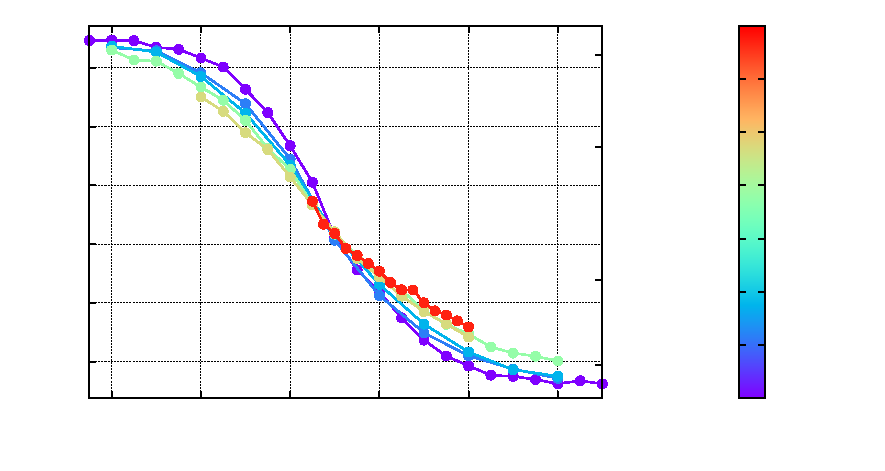
\includegraphics{KiskerTransmissionCalibration}}%
    \gplfronttext
  \end{picture}%
\endgroup

		\caption[Calibration of the solvent electron density by X-ray transmission.]{Solvent density along the gradient capillary vertical axis at different diffusion times, calculated from the transmission measurements at 5500 eV of 100 nm polystyrene particles. The corresponding X-ray transmission is shown on the right axis, revealing the low transmittances of the filled capillary at low energies.}
		\label{fig:KiskerTransmissionCalibration}
\end{figure*}

The X-ray transmission measurements are performed at a low incident photon energy of $E = 5500$ eV to increase the transmittance differences for the less absorbing sucrose solution. In figure \ref{fig:EnergiesTransmissionCalibration}, the calculated transmittances of a 65 $\%$ concentrated sucrose mixture and water (0 $\%$) are depicted, along with the ratio between both transmissions. This ratio decreases for high energies, suppressing the transmission differences between both components of the density gradient column. This fact is revealed in figure \ref{fig:SucroseTransmissionCalibration}, where the X-ray transmittance of an aqueous sucrose density gradient measured at 5500 eV shows a better signal-to-noise ratio than the same measurement at 10000 eV.

\begin{figure*}%[htbp]
	\centering
                \subfloat[Calculated transmittance]{\resizebox{0.44\linewidth}{!}{\figfont{13pt}% GNUPLOT: LaTeX picture with Postscript
\begingroup
  \makeatletter
  \providecommand\color[2][]{%
    \GenericError{(gnuplot) \space\space\space\@spaces}{%
      Package color not loaded in conjunction with
      terminal option `colourtext'%
    }{See the gnuplot documentation for explanation.%
    }{Either use 'blacktext' in gnuplot or load the package
      color.sty in LaTeX.}%
    \renewcommand\color[2][]{}%
  }%
  \providecommand\includegraphics[2][]{%
    \GenericError{(gnuplot) \space\space\space\@spaces}{%
      Package graphicx or graphics not loaded%
    }{See the gnuplot documentation for explanation.%
    }{The gnuplot epslatex terminal needs graphicx.sty or graphics.sty.}%
    \renewcommand\includegraphics[2][]{}%
  }%
  \providecommand\rotatebox[2]{#2}%
  \@ifundefined{ifGPcolor}{%
    \newif\ifGPcolor
    \GPcolortrue
  }{}%
  \@ifundefined{ifGPblacktext}{%
    \newif\ifGPblacktext
    \GPblacktextfalse
  }{}%
  % define a \g@addto@macro without @ in the name:
  \let\gplgaddtomacro\g@addto@macro
  % define empty templates for all commands taking text:
  \gdef\gplbacktext{}%
  \gdef\gplfronttext{}%
  \makeatother
  \ifGPblacktext
    % no textcolor at all
    \def\colorrgb#1{}%
    \def\colorgray#1{}%
  \else
    % gray or color?
    \ifGPcolor
      \def\colorrgb#1{\color[rgb]{#1}}%
      \def\colorgray#1{\color[gray]{#1}}%
      \expandafter\def\csname LTw\endcsname{\color{white}}%
      \expandafter\def\csname LTb\endcsname{\color{black}}%
      \expandafter\def\csname LTa\endcsname{\color{black}}%
      \expandafter\def\csname LT0\endcsname{\color[rgb]{1,0,0}}%
      \expandafter\def\csname LT1\endcsname{\color[rgb]{0,1,0}}%
      \expandafter\def\csname LT2\endcsname{\color[rgb]{0,0,1}}%
      \expandafter\def\csname LT3\endcsname{\color[rgb]{1,0,1}}%
      \expandafter\def\csname LT4\endcsname{\color[rgb]{0,1,1}}%
      \expandafter\def\csname LT5\endcsname{\color[rgb]{1,1,0}}%
      \expandafter\def\csname LT6\endcsname{\color[rgb]{0,0,0}}%
      \expandafter\def\csname LT7\endcsname{\color[rgb]{1,0.3,0}}%
      \expandafter\def\csname LT8\endcsname{\color[rgb]{0.5,0.5,0.5}}%
    \else
      % gray
      \def\colorrgb#1{\color{black}}%
      \def\colorgray#1{\color[gray]{#1}}%
      \expandafter\def\csname LTw\endcsname{\color{white}}%
      \expandafter\def\csname LTb\endcsname{\color{black}}%
      \expandafter\def\csname LTa\endcsname{\color{black}}%
      \expandafter\def\csname LT0\endcsname{\color{black}}%
      \expandafter\def\csname LT1\endcsname{\color{black}}%
      \expandafter\def\csname LT2\endcsname{\color{black}}%
      \expandafter\def\csname LT3\endcsname{\color{black}}%
      \expandafter\def\csname LT4\endcsname{\color{black}}%
      \expandafter\def\csname LT5\endcsname{\color{black}}%
      \expandafter\def\csname LT6\endcsname{\color{black}}%
      \expandafter\def\csname LT7\endcsname{\color{black}}%
      \expandafter\def\csname LT8\endcsname{\color{black}}%
    \fi
  \fi
  \setlength{\unitlength}{0.0500bp}%
  \begin{picture}(5668.00,4534.00)%
    \gplgaddtomacro\gplbacktext{%
      \csname LTb\endcsname%
      \put(946,939){\makebox(0,0)[r]{\strut{} 0.1}}%
      \csname LTb\endcsname%
      \put(946,2109){\makebox(0,0)[r]{\strut{} 1}}%
      \csname LTb\endcsname%
      \put(946,3280){\makebox(0,0)[r]{\strut{} 10}}%
      \csname LTb\endcsname%
      \put(1078,484){\makebox(0,0){\strut{} 5000}}%
      \csname LTb\endcsname%
      \put(1741,484){\makebox(0,0){\strut{} 6000}}%
      \csname LTb\endcsname%
      \put(2403,484){\makebox(0,0){\strut{} 7000}}%
      \csname LTb\endcsname%
      \put(3066,484){\makebox(0,0){\strut{} 8000}}%
      \csname LTb\endcsname%
      \put(3728,484){\makebox(0,0){\strut{} 9000}}%
      \csname LTb\endcsname%
      \put(4391,484){\makebox(0,0){\strut{} 10000}}%
      \colorrgb{0.00,0.00,1.00}%
      \put(4523,1224){\makebox(0,0)[l]{\strut{} 1.5}}%
      \colorrgb{0.00,0.00,1.00}%
      \put(4523,1967){\makebox(0,0)[l]{\strut{} 2}}%
      \colorrgb{0.00,0.00,1.00}%
      \put(4523,2709){\makebox(0,0)[l]{\strut{} 2.5}}%
      \colorrgb{0.00,0.00,1.00}%
      \put(4523,3452){\makebox(0,0)[l]{\strut{} 3}}%
      \colorrgb{0.00,0.00,1.00}%
      \put(4523,4195){\makebox(0,0)[l]{\strut{} 3.5}}%
      \csname LTb\endcsname%
      \put(176,2486){\rotatebox{-270}{\makebox(0,0){\strut{}X-ray Transmission / $\%$}}}%
      \colorrgb{0.00,0.00,1.00}%
      \put(5160,2486){\rotatebox{270}{\makebox(0,0){\strut{}Ratio}}}%
      \csname LTb\endcsname%
      \put(2734,154){\makebox(0,0){\strut{}Energy / eV}}%
    }%
    \gplgaddtomacro\gplfronttext{%
      \csname LTb\endcsname%
      \put(3800,2649){\makebox(0,0)[r]{\strut{}\smaller Capillary}}%
      \csname LTb\endcsname%
      \put(3800,2319){\makebox(0,0)[r]{\strut{}\smaller 0$\%$ sucrose}}%
      \csname LTb\endcsname%
      \put(3800,1989){\makebox(0,0)[r]{\strut{}\smaller 65$\%$ sucrose}}%
      \csname LTb\endcsname%
      \put(3800,1659){\makebox(0,0)[r]{\strut{}\smaller T$_{0\%}$/T$_{65\%}$}}%
    }%
    \gplbacktext
    \put(0,0){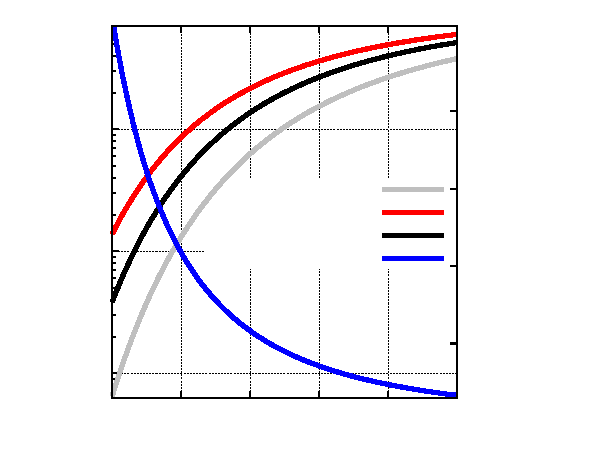
\includegraphics{EnergiesTransmissionCalibration}}%
    \gplfronttext
  \end{picture}%
\endgroup
}\label{fig:EnergiesTransmissionCalibration}}
		\subfloat[Calibrated sucrose concentration]{\resizebox{0.44\linewidth}{!}{\figfont{13pt}% GNUPLOT: LaTeX picture with Postscript
\begingroup
  \makeatletter
  \providecommand\color[2][]{%
    \GenericError{(gnuplot) \space\space\space\@spaces}{%
      Package color not loaded in conjunction with
      terminal option `colourtext'%
    }{See the gnuplot documentation for explanation.%
    }{Either use 'blacktext' in gnuplot or load the package
      color.sty in LaTeX.}%
    \renewcommand\color[2][]{}%
  }%
  \providecommand\includegraphics[2][]{%
    \GenericError{(gnuplot) \space\space\space\@spaces}{%
      Package graphicx or graphics not loaded%
    }{See the gnuplot documentation for explanation.%
    }{The gnuplot epslatex terminal needs graphicx.sty or graphics.sty.}%
    \renewcommand\includegraphics[2][]{}%
  }%
  \providecommand\rotatebox[2]{#2}%
  \@ifundefined{ifGPcolor}{%
    \newif\ifGPcolor
    \GPcolortrue
  }{}%
  \@ifundefined{ifGPblacktext}{%
    \newif\ifGPblacktext
    \GPblacktextfalse
  }{}%
  % define a \g@addto@macro without @ in the name:
  \let\gplgaddtomacro\g@addto@macro
  % define empty templates for all commands taking text:
  \gdef\gplbacktext{}%
  \gdef\gplfronttext{}%
  \makeatother
  \ifGPblacktext
    % no textcolor at all
    \def\colorrgb#1{}%
    \def\colorgray#1{}%
  \else
    % gray or color?
    \ifGPcolor
      \def\colorrgb#1{\color[rgb]{#1}}%
      \def\colorgray#1{\color[gray]{#1}}%
      \expandafter\def\csname LTw\endcsname{\color{white}}%
      \expandafter\def\csname LTb\endcsname{\color{black}}%
      \expandafter\def\csname LTa\endcsname{\color{black}}%
      \expandafter\def\csname LT0\endcsname{\color[rgb]{1,0,0}}%
      \expandafter\def\csname LT1\endcsname{\color[rgb]{0,1,0}}%
      \expandafter\def\csname LT2\endcsname{\color[rgb]{0,0,1}}%
      \expandafter\def\csname LT3\endcsname{\color[rgb]{1,0,1}}%
      \expandafter\def\csname LT4\endcsname{\color[rgb]{0,1,1}}%
      \expandafter\def\csname LT5\endcsname{\color[rgb]{1,1,0}}%
      \expandafter\def\csname LT6\endcsname{\color[rgb]{0,0,0}}%
      \expandafter\def\csname LT7\endcsname{\color[rgb]{1,0.3,0}}%
      \expandafter\def\csname LT8\endcsname{\color[rgb]{0.5,0.5,0.5}}%
    \else
      % gray
      \def\colorrgb#1{\color{black}}%
      \def\colorgray#1{\color[gray]{#1}}%
      \expandafter\def\csname LTw\endcsname{\color{white}}%
      \expandafter\def\csname LTb\endcsname{\color{black}}%
      \expandafter\def\csname LTa\endcsname{\color{black}}%
      \expandafter\def\csname LT0\endcsname{\color{black}}%
      \expandafter\def\csname LT1\endcsname{\color{black}}%
      \expandafter\def\csname LT2\endcsname{\color{black}}%
      \expandafter\def\csname LT3\endcsname{\color{black}}%
      \expandafter\def\csname LT4\endcsname{\color{black}}%
      \expandafter\def\csname LT5\endcsname{\color{black}}%
      \expandafter\def\csname LT6\endcsname{\color{black}}%
      \expandafter\def\csname LT7\endcsname{\color{black}}%
      \expandafter\def\csname LT8\endcsname{\color{black}}%
    \fi
  \fi
  \setlength{\unitlength}{0.0500bp}%
  \begin{picture}(5668.00,4534.00)%
    \gplgaddtomacro\gplbacktext{%
      \csname LTb\endcsname%
      \put(814,942){\makebox(0,0)[r]{\strut{} 0}}%
      \csname LTb\endcsname%
      \put(814,1417){\makebox(0,0)[r]{\strut{} 10}}%
      \csname LTb\endcsname%
      \put(814,1892){\makebox(0,0)[r]{\strut{} 20}}%
      \csname LTb\endcsname%
      \put(814,2368){\makebox(0,0)[r]{\strut{} 30}}%
      \csname LTb\endcsname%
      \put(814,2843){\makebox(0,0)[r]{\strut{} 40}}%
      \csname LTb\endcsname%
      \put(814,3318){\makebox(0,0)[r]{\strut{} 50}}%
      \csname LTb\endcsname%
      \put(814,3794){\makebox(0,0)[r]{\strut{} 60}}%
      \csname LTb\endcsname%
      \put(814,4269){\makebox(0,0)[r]{\strut{} 70}}%
      \csname LTb\endcsname%
      \put(946,484){\makebox(0,0){\strut{} 0}}%
      \csname LTb\endcsname%
      \put(2027,484){\makebox(0,0){\strut{} 5}}%
      \csname LTb\endcsname%
      \put(3109,484){\makebox(0,0){\strut{} 10}}%
      \csname LTb\endcsname%
      \put(4190,484){\makebox(0,0){\strut{} 15}}%
      \csname LTb\endcsname%
      \put(5271,484){\makebox(0,0){\strut{} 20}}%
      \put(176,2486){\rotatebox{-270}{\makebox(0,0){\strut{}Sucrose Mass Fraction / $\%$}}}%
      \put(3108,154){\makebox(0,0){\strut{}Vertical Position / mm}}%
    }%
    \gplgaddtomacro\gplfronttext{%
      \csname LTb\endcsname%
      \put(4284,4096){\makebox(0,0)[r]{\strut{}5500 eV}}%
      \csname LTb\endcsname%
      \put(4284,3876){\makebox(0,0)[r]{\strut{}8000 eV}}%
      \csname LTb\endcsname%
      \put(4284,3656){\makebox(0,0)[r]{\strut{}10000 eV}}%
    }%
    \gplbacktext
    \put(0,0){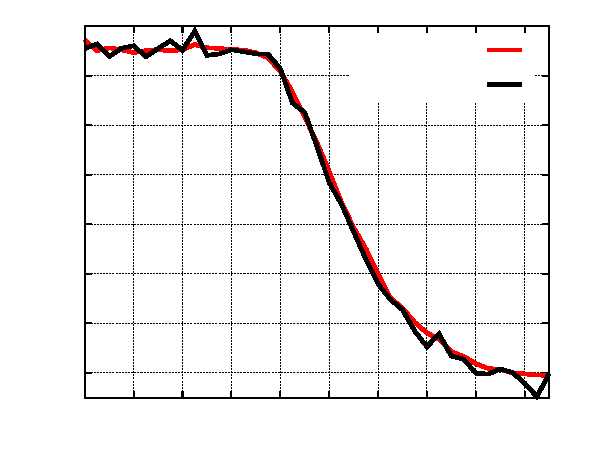
\includegraphics{SucroseTransmissionCalibration}}%
    \gplfronttext
  \end{picture}%
\endgroup
}\label{fig:SucroseTransmissionCalibration}}
	\caption[X-ray transmittance of the density gradient capillary at different energies.]{X-ray transmittance as a function of the photon energy. a) Calculated transmittances \citep{henke_x-ray_1993} of an empty capillary, water and an aqueous sucrose mixture with 65 $\%$ mass fraction assuming a 1 mm sample thickness and the nominal specifications of the glass capillary. The ratio between the water and the sucrose mixture transmittances is shown in the right axis. b) Sucrose mass fraction derived from an experimental transmittance measurement of a 65 $\%$ sucrose density gradient measured at two different energies under similar experimental conditions. The absorbance differences are smaller for the higher energy.}

\end{figure*}

The calculated transmission of the empty rectangular capillary is less than 1 $\%$ below 6000 eV as shown in figure \ref{fig:EnergiesTransmissionCalibration} and the filled capillary just transmits 0.03 $\%$ of the incoming photon flux at 5500 eV, as observed in figure \ref{fig:KiskerTransmissionCalibration}. Therefore, a compromise between the absorbance ratio and the capillary transmittance is taken at a photon energy of 5500 eV. 

\subsection{SAXS measurements}
\label{sec:DensityGradientSAXS}

In order to collect the scattering patterns, the sample is moved in steps of 0.5 mm along the central vertical capillary axis and exposed at each position for about 1 minute. The acquisition time depends notably on the experimental parameters (e.g. sample concentration, scattering power of the material...), though it is strictly limited by the diffusion time of the contrast agent. At these positions, the solution transmittances were previously measured and the suspending medium electron density calibrated, as described previously. Due to a vertical beam size of about 0.5 mm, the measured scattering curve is an average over a range of solvent electron densities, specially relevant at the height where the density gradient is steeper. 

As a consequence of the observations from figure \ref{fig:EnergiesTransmissionCalibration}, the incident photon energy \(E = \left(8000.0  \pm 0.8\right)\) eV was chosen to be higher than the photon energy employed for the transmission measurements to improve the recorded statistics, due to a ca. 200 higher transmission \citep{henke_x-ray_1993}. On the other hand, the decreasing photon flux at the FCM beamline for high energies as depicted in figure \ref{fig:FCMBeamlineFlux}, suggest the utilization of photon energies below 8800 eV in scattering experiments.

The dimensions of the investigated particle defines the required $q$-range of the experiment, which is delimited by the photon energy and the sample-detector distance, as discussed in section \ref{sec:SAXS_experimental}. The photon energy is generally limited by the needs of the sample environment, but the distance can be adjusted with the HZB-SAXS instrument to the nanoparticle requirements and can compensate the energy restriction. For sizes typically ranging from 10 to 200 nm, the sample-detector distance is fixed at 4500 mm and enables $q$-values between 0.03 and 1.1 nm$^{-1}$ at 8000 eV.

Since the installation in April 2016 of the monitor diode on the beamstop presented in section \ref{sec:pilatus}, the sample transmittance can be recorded simultaneously with the scattering patterns. The longer integration times required for the scattering experiments (around 60 s) increase by a factor 6 the statistics of the simultaneous X-ray transmission measurement, improving the quality of the transmittance data. The possibility to collect the scattering data at the same photon energy that the solution transmittances improves the normalization of the scattering curve and the calibration of the solvent electron densities. Unfortunately, all the results presented in this work were recorded before the commissioning of the beamstop diode.

\section{Proof of principle: Application to the PS-COOH particles}
\label{sec:KiskerResults}

In order to demonstrate the proposed continuous contrast variation technique, carboxylated polystyrene nanoparticles with a nominal size of 105 nm suspended in water (Kisker, Steinfurt, Germany) were measured following the procedure described previously in this chapter. The particles have a narrow size distribution and consist of a spherical polystyrene (PS) core enclosed by a thin shell of a denser polymer, most likely poly(methyl methacrylate) (PMMA). The synthesis by multi-addition emulsion polymerization is responsible of the core-shell structure found in these PS-COOH particles and suggests that all the particles have the same average density independent on their size.

\begin{figure}%[htbp]
	\centering
		% GNUPLOT: LaTeX picture with Postscript
\begingroup
  \makeatletter
  \providecommand\color[2][]{%
    \GenericError{(gnuplot) \space\space\space\@spaces}{%
      Package color not loaded in conjunction with
      terminal option `colourtext'%
    }{See the gnuplot documentation for explanation.%
    }{Either use 'blacktext' in gnuplot or load the package
      color.sty in LaTeX.}%
    \renewcommand\color[2][]{}%
  }%
  \providecommand\includegraphics[2][]{%
    \GenericError{(gnuplot) \space\space\space\@spaces}{%
      Package graphicx or graphics not loaded%
    }{See the gnuplot documentation for explanation.%
    }{The gnuplot epslatex terminal needs graphicx.sty or graphics.sty.}%
    \renewcommand\includegraphics[2][]{}%
  }%
  \providecommand\rotatebox[2]{#2}%
  \@ifundefined{ifGPcolor}{%
    \newif\ifGPcolor
    \GPcolortrue
  }{}%
  \@ifundefined{ifGPblacktext}{%
    \newif\ifGPblacktext
    \GPblacktextfalse
  }{}%
  % define a \g@addto@macro without @ in the name:
  \let\gplgaddtomacro\g@addto@macro
  % define empty templates for all commands taking text:
  \gdef\gplbacktext{}%
  \gdef\gplfronttext{}%
  \makeatother
  \ifGPblacktext
    % no textcolor at all
    \def\colorrgb#1{}%
    \def\colorgray#1{}%
  \else
    % gray or color?
    \ifGPcolor
      \def\colorrgb#1{\color[rgb]{#1}}%
      \def\colorgray#1{\color[gray]{#1}}%
      \expandafter\def\csname LTw\endcsname{\color{white}}%
      \expandafter\def\csname LTb\endcsname{\color{black}}%
      \expandafter\def\csname LTa\endcsname{\color{black}}%
      \expandafter\def\csname LT0\endcsname{\color[rgb]{1,0,0}}%
      \expandafter\def\csname LT1\endcsname{\color[rgb]{0,1,0}}%
      \expandafter\def\csname LT2\endcsname{\color[rgb]{0,0,1}}%
      \expandafter\def\csname LT3\endcsname{\color[rgb]{1,0,1}}%
      \expandafter\def\csname LT4\endcsname{\color[rgb]{0,1,1}}%
      \expandafter\def\csname LT5\endcsname{\color[rgb]{1,1,0}}%
      \expandafter\def\csname LT6\endcsname{\color[rgb]{0,0,0}}%
      \expandafter\def\csname LT7\endcsname{\color[rgb]{1,0.3,0}}%
      \expandafter\def\csname LT8\endcsname{\color[rgb]{0.5,0.5,0.5}}%
    \else
      % gray
      \def\colorrgb#1{\color{black}}%
      \def\colorgray#1{\color[gray]{#1}}%
      \expandafter\def\csname LTw\endcsname{\color{white}}%
      \expandafter\def\csname LTb\endcsname{\color{black}}%
      \expandafter\def\csname LTa\endcsname{\color{black}}%
      \expandafter\def\csname LT0\endcsname{\color{black}}%
      \expandafter\def\csname LT1\endcsname{\color{black}}%
      \expandafter\def\csname LT2\endcsname{\color{black}}%
      \expandafter\def\csname LT3\endcsname{\color{black}}%
      \expandafter\def\csname LT4\endcsname{\color{black}}%
      \expandafter\def\csname LT5\endcsname{\color{black}}%
      \expandafter\def\csname LT6\endcsname{\color{black}}%
      \expandafter\def\csname LT7\endcsname{\color{black}}%
      \expandafter\def\csname LT8\endcsname{\color{black}}%
    \fi
  \fi
  \setlength{\unitlength}{0.0500bp}%
  \begin{picture}(5668.00,4534.00)%
    \gplgaddtomacro\gplbacktext{%
      \csname LTb\endcsname%
      \put(858,937){\makebox(0,0)[r]{\strut{} 1}}%
      \csname LTb\endcsname%
      \put(858,1986){\makebox(0,0)[r]{\strut{} 10}}%
      \csname LTb\endcsname%
      \put(858,3035){\makebox(0,0)[r]{\strut{} 100}}%
      \csname LTb\endcsname%
      \put(858,4084){\makebox(0,0)[r]{\strut{} 1000}}%
      \csname LTb\endcsname%
      \put(990,484){\makebox(0,0){\strut{} 0.03}}%
      \csname LTb\endcsname%
      \put(1615,484){\makebox(0,0){\strut{} 0.05}}%
      \csname LTb\endcsname%
      \put(2463,484){\makebox(0,0){\strut{} 0.1}}%
      \csname LTb\endcsname%
      \put(3312,484){\makebox(0,0){\strut{} 0.2}}%
      \csname LTb\endcsname%
      \put(3808,484){\makebox(0,0){\strut{} 0.3}}%
      \csname LTb\endcsname%
      \put(4433,484){\makebox(0,0){\strut{} 0.5}}%
      \put(220,2266){\rotatebox{-270}{\makebox(0,0){\strut{}Scattering Intensity / a.u.}}}%
      \put(2711,154){\makebox(0,0){\strut{}$q$ / nm$^{-1}$}}%
    }%
    \gplgaddtomacro\gplfronttext{%
      \csname LTb\endcsname%
      \put(4692,878){\makebox(0,0)[l]{\strut{}335.0}}%
      \put(4692,1548){\makebox(0,0)[l]{\strut{}340.0}}%
      \put(4692,2218){\makebox(0,0)[l]{\strut{}345.0}}%
      \put(4692,2888){\makebox(0,0)[l]{\strut{}350.0}}%
      \put(4692,3558){\makebox(0,0)[l]{\strut{}355.0}}%
      \put(4692,4228){\makebox(0,0)[l]{\strut{}360.0}}%
      \put(5418,2486){\rotatebox{-90}{\makebox(0,0){\strut{}\fsmedium Solvent Electron Density / nm$^{-3}$}}}%
    }%
    \gplbacktext
    \put(0,0){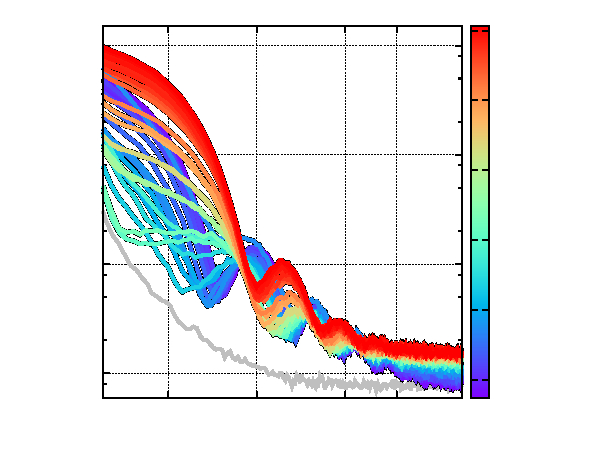
\includegraphics{KiskerContinuousSAXS}}%
    \gplfronttext
  \end{picture}%
\endgroup

		\caption[Experimental scattering curves of the PS-COOH particles for different suspending medium electron densities.]{Experimental scattering curves of the PS-COOH nanoparticles for different suspending medium electron densities measured between 78 and 93 minutes after the inception of the density gradient. The gray line shows the experimental background, containing scattering contributions from the capillary and the pure solvent.}
		\label{fig:KiskerContinuousSAXS}
\end{figure}

The density gradient capillary was built according to the description in section \ref{sec:GradientPreparation} using two aqueous mixtures with a particle concentration of 12.6 mg ml$^{-1}$ according to the producer's specification. The dense aqueous solution was prepared with 21.23 $\%$ sucrose mass fraction with a mass density of \(\rho_1=1.088 \) g cm$^{-3}$, whereas a lighter one was produced without sucrose (\(\rho_2=0.997 \) g cm$^{-3}$). In total, 40 scattering curves with different solvent electron densities were measured at two different times \(t_1=\)78 min and \(t_2=\)156 min after filling the capillaries.

The measured scattering curves of the PS-COOH particles are displayed in figure \ref{fig:KiskerContinuousSAXS}. In the region for \(q\) from 0.03 nm\(^{-1}\) to 0.5 nm\(^{-1}\) it is possible to observe the variation of the curve features corresponding to the particle form factor through the increase of the solvent electron density from 333.7 nm\(^{-3}\) at the top edge of the density gradient to 360.3 nm\(^{-3}\) at the maximum sucrose concentration. In this region, the experimental background is composed mainly by the contribution of the capillary scattering at the low $q$-region and the uniform scattering of the suspending medium. The experimental background scattering varies for different sucrose concentrations, but their variations are small and the background remains one order of magnitude below the sample scattering in the relevant Fourier region.

Upon increasing the solvent density, the position of the first minimum shifts from 0.07 nm\(^{-1}\) towards smaller \(q\)-values until it vanishes when the solvent electron density matches the average electron density of the measured particle. In the Fourier region of the scattering curves, several minima are observed which shift towards smaller \(q\)-values when increasing the solvent electron density. Upon subtracting the experimental background from the scattering curve, a decrease of the scattering intensity towards $q=0$ is observed only for the solvent electron density closest to the match point as depicted in figure \ref{fig:KiskerBackgroundSubtraction}. Therefore, background corrections can be neglected for systems with relatively high scattering power like in this study. For low-scatterers, an accurate background correction by measuring the pure suspending medium at different sucrose concentrations might be required. The behaviour at low $q$-values will be further discussed in section \ref{sec:guinier_analysis} when evaluating the zero-angle intensity.

\begin{figure}%[htbp]
	\centering
		% GNUPLOT: LaTeX picture with Postscript
\begingroup
  \makeatletter
  \providecommand\color[2][]{%
    \GenericError{(gnuplot) \space\space\space\@spaces}{%
      Package color not loaded in conjunction with
      terminal option `colourtext'%
    }{See the gnuplot documentation for explanation.%
    }{Either use 'blacktext' in gnuplot or load the package
      color.sty in LaTeX.}%
    \renewcommand\color[2][]{}%
  }%
  \providecommand\includegraphics[2][]{%
    \GenericError{(gnuplot) \space\space\space\@spaces}{%
      Package graphicx or graphics not loaded%
    }{See the gnuplot documentation for explanation.%
    }{The gnuplot epslatex terminal needs graphicx.sty or graphics.sty.}%
    \renewcommand\includegraphics[2][]{}%
  }%
  \providecommand\rotatebox[2]{#2}%
  \@ifundefined{ifGPcolor}{%
    \newif\ifGPcolor
    \GPcolortrue
  }{}%
  \@ifundefined{ifGPblacktext}{%
    \newif\ifGPblacktext
    \GPblacktextfalse
  }{}%
  % define a \g@addto@macro without @ in the name:
  \let\gplgaddtomacro\g@addto@macro
  % define empty templates for all commands taking text:
  \gdef\gplbacktext{}%
  \gdef\gplfronttext{}%
  \makeatother
  \ifGPblacktext
    % no textcolor at all
    \def\colorrgb#1{}%
    \def\colorgray#1{}%
  \else
    % gray or color?
    \ifGPcolor
      \def\colorrgb#1{\color[rgb]{#1}}%
      \def\colorgray#1{\color[gray]{#1}}%
      \expandafter\def\csname LTw\endcsname{\color{white}}%
      \expandafter\def\csname LTb\endcsname{\color{black}}%
      \expandafter\def\csname LTa\endcsname{\color{black}}%
      \expandafter\def\csname LT0\endcsname{\color[rgb]{1,0,0}}%
      \expandafter\def\csname LT1\endcsname{\color[rgb]{0,1,0}}%
      \expandafter\def\csname LT2\endcsname{\color[rgb]{0,0,1}}%
      \expandafter\def\csname LT3\endcsname{\color[rgb]{1,0,1}}%
      \expandafter\def\csname LT4\endcsname{\color[rgb]{0,1,1}}%
      \expandafter\def\csname LT5\endcsname{\color[rgb]{1,1,0}}%
      \expandafter\def\csname LT6\endcsname{\color[rgb]{0,0,0}}%
      \expandafter\def\csname LT7\endcsname{\color[rgb]{1,0.3,0}}%
      \expandafter\def\csname LT8\endcsname{\color[rgb]{0.5,0.5,0.5}}%
    \else
      % gray
      \def\colorrgb#1{\color{black}}%
      \def\colorgray#1{\color[gray]{#1}}%
      \expandafter\def\csname LTw\endcsname{\color{white}}%
      \expandafter\def\csname LTb\endcsname{\color{black}}%
      \expandafter\def\csname LTa\endcsname{\color{black}}%
      \expandafter\def\csname LT0\endcsname{\color{black}}%
      \expandafter\def\csname LT1\endcsname{\color{black}}%
      \expandafter\def\csname LT2\endcsname{\color{black}}%
      \expandafter\def\csname LT3\endcsname{\color{black}}%
      \expandafter\def\csname LT4\endcsname{\color{black}}%
      \expandafter\def\csname LT5\endcsname{\color{black}}%
      \expandafter\def\csname LT6\endcsname{\color{black}}%
      \expandafter\def\csname LT7\endcsname{\color{black}}%
      \expandafter\def\csname LT8\endcsname{\color{black}}%
    \fi
  \fi
  \setlength{\unitlength}{0.0500bp}%
  \begin{picture}(5668.00,4534.00)%
    \gplgaddtomacro\gplbacktext{%
      \csname LTb\endcsname%
      \put(594,1636){\makebox(0,0)[r]{\strut{} 1}}%
      \csname LTb\endcsname%
      \put(594,3419){\makebox(0,0)[r]{\strut{} 10}}%
      \csname LTb\endcsname%
      \put(1315,484){\makebox(0,0){\strut{} 0.05}}%
      \csname LTb\endcsname%
      \put(2231,484){\makebox(0,0){\strut{} 0.1}}%
      \csname LTb\endcsname%
      \put(3146,484){\makebox(0,0){\strut{} 0.2}}%
      \csname LTb\endcsname%
      \put(4356,484){\makebox(0,0){\strut{} 0.5}}%
      \csname LTb\endcsname%
      \put(5271,484){\makebox(0,0){\strut{} 1}}%
      \put(220,2266){\rotatebox{-270}{\makebox(0,0){\strut{}Scattering Intensity / a.u.}}}%
      \put(2998,154){\makebox(0,0){\strut{}$q$ / nm$^{-1}$}}%
    }%
    \gplgaddtomacro\gplfronttext{%
      \csname LTb\endcsname%
      \put(4284,4096){\makebox(0,0)[r]{\strut{}Original curve}}%
      \csname LTb\endcsname%
      \put(4284,3876){\makebox(0,0)[r]{\strut{}Water Background}}%
      \csname LTb\endcsname%
      \put(4284,3656){\makebox(0,0)[r]{\strut{}Subtracted Curve}}%
    }%
    \gplbacktext
    \put(0,0){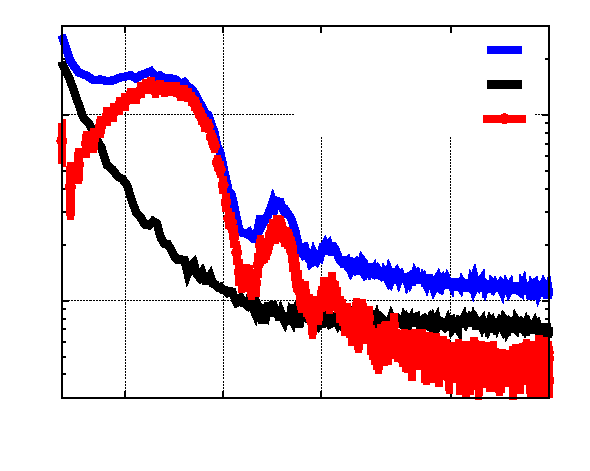
\includegraphics{KiskerBackgroundSubtraction}}%
    \gplfronttext
  \end{picture}%
\endgroup

		\caption[Background subtraction of the scattering curves of the PS-COOH particles.]{The thick blue line shows the scattering curve measured at $\rho_{\text{solv}}$ = 345.4 nm$^{-3}$, close to the match point, and the black line displays the experimental background. The red symbols with errorbars show the background corrected scattering curve.}
		\label{fig:KiskerBackgroundSubtraction}
\end{figure}

The presence of the clearly visible isoscattering point around \(q=0.09\) nm\(^{-1}\) confirms the existence of an inner structure. This heterogeneous composition was previously reported for the same colloids by \citet{minelli_characterization_2014}, who observed methacrylic acid (MAA) and methylmethacrylate (MMA) at the particle surface, both monomer precursors of PMMA polymerization. A more detailed insight into the radial morphology is presented subsequently, using the theoretical framework introduced in chapter \ref{chap:theory_SAXS}.

\section{Results and data evaluation}
\label{sec:KiskerResultsEvaluation}

The scattering curves of the PS-COOH nanoparticles measured at several contrasts can be analysed using different, complementary evaluation methods. In this section, both a model-free theoretical framework as well as a core-shell model fit are applied and, in combination, deliver a detailed insight into the inner structure of particles.


\subsection{Core-shell form factor fit}
\label{sec:coreshell_fit}
A core-shell model fit to the scattering curves is displayed in figure \ref{fig:KiskerSAXSCoreshellFit} for three representative contrasts, which employs the form factor described by expression \ref{eq:ff_cs}. The simultaneous fitting of the form factor to the 40 measured scattering curves was performed by means of the method of least squares in the Fourier region \citep{pedersen_analysis_1997}. The calculated scattered intensity was modelled as the sum of the particle contributions and a two-component background \(I_{\text{BG}}=C_0+C_4q^{-\gamma} \). The parameters \(\rho_{\text{core}}\), \(\rho_{\text{shell}}\), \(R\), \(R_{\text{core}}\) and \(\gamma\) were fitted simultaneously for all curves, whilst \( C_0 \) and \( C_4 \) were adjusted independently for each solvent density. A Gaussian size distribution was assumed. For the suspending medium electron density \( \rho_{\text{solv}} \) appearing in the contrast \( \Delta\eta \), the value determined from the transmission measurement was used for each curve.

\begin{figure}%[htbp]
	\centering
		% GNUPLOT: LaTeX picture with Postscript
\begingroup
  \makeatletter
  \providecommand\color[2][]{%
    \GenericError{(gnuplot) \space\space\space\@spaces}{%
      Package color not loaded in conjunction with
      terminal option `colourtext'%
    }{See the gnuplot documentation for explanation.%
    }{Either use 'blacktext' in gnuplot or load the package
      color.sty in LaTeX.}%
    \renewcommand\color[2][]{}%
  }%
  \providecommand\includegraphics[2][]{%
    \GenericError{(gnuplot) \space\space\space\@spaces}{%
      Package graphicx or graphics not loaded%
    }{See the gnuplot documentation for explanation.%
    }{The gnuplot epslatex terminal needs graphicx.sty or graphics.sty.}%
    \renewcommand\includegraphics[2][]{}%
  }%
  \providecommand\rotatebox[2]{#2}%
  \@ifundefined{ifGPcolor}{%
    \newif\ifGPcolor
    \GPcolortrue
  }{}%
  \@ifundefined{ifGPblacktext}{%
    \newif\ifGPblacktext
    \GPblacktextfalse
  }{}%
  % define a \g@addto@macro without @ in the name:
  \let\gplgaddtomacro\g@addto@macro
  % define empty templates for all commands taking text:
  \gdef\gplbacktext{}%
  \gdef\gplfronttext{}%
  \makeatother
  \ifGPblacktext
    % no textcolor at all
    \def\colorrgb#1{}%
    \def\colorgray#1{}%
  \else
    % gray or color?
    \ifGPcolor
      \def\colorrgb#1{\color[rgb]{#1}}%
      \def\colorgray#1{\color[gray]{#1}}%
      \expandafter\def\csname LTw\endcsname{\color{white}}%
      \expandafter\def\csname LTb\endcsname{\color{black}}%
      \expandafter\def\csname LTa\endcsname{\color{black}}%
      \expandafter\def\csname LT0\endcsname{\color[rgb]{1,0,0}}%
      \expandafter\def\csname LT1\endcsname{\color[rgb]{0,1,0}}%
      \expandafter\def\csname LT2\endcsname{\color[rgb]{0,0,1}}%
      \expandafter\def\csname LT3\endcsname{\color[rgb]{1,0,1}}%
      \expandafter\def\csname LT4\endcsname{\color[rgb]{0,1,1}}%
      \expandafter\def\csname LT5\endcsname{\color[rgb]{1,1,0}}%
      \expandafter\def\csname LT6\endcsname{\color[rgb]{0,0,0}}%
      \expandafter\def\csname LT7\endcsname{\color[rgb]{1,0.3,0}}%
      \expandafter\def\csname LT8\endcsname{\color[rgb]{0.5,0.5,0.5}}%
    \else
      % gray
      \def\colorrgb#1{\color{black}}%
      \def\colorgray#1{\color[gray]{#1}}%
      \expandafter\def\csname LTw\endcsname{\color{white}}%
      \expandafter\def\csname LTb\endcsname{\color{black}}%
      \expandafter\def\csname LTa\endcsname{\color{black}}%
      \expandafter\def\csname LT0\endcsname{\color{black}}%
      \expandafter\def\csname LT1\endcsname{\color{black}}%
      \expandafter\def\csname LT2\endcsname{\color{black}}%
      \expandafter\def\csname LT3\endcsname{\color{black}}%
      \expandafter\def\csname LT4\endcsname{\color{black}}%
      \expandafter\def\csname LT5\endcsname{\color{black}}%
      \expandafter\def\csname LT6\endcsname{\color{black}}%
      \expandafter\def\csname LT7\endcsname{\color{black}}%
      \expandafter\def\csname LT8\endcsname{\color{black}}%
    \fi
  \fi
    \setlength{\unitlength}{0.0500bp}%
    \ifx\gptboxheight\undefined%
      \newlength{\gptboxheight}%
      \newlength{\gptboxwidth}%
      \newsavebox{\gptboxtext}%
    \fi%
    \setlength{\fboxrule}{0.5pt}%
    \setlength{\fboxsep}{1pt}%
\begin{picture}(5668.00,4534.00)%
    \gplgaddtomacro\gplbacktext{%
      \csname LTb\endcsname%
      \put(726,1013){\makebox(0,0)[r]{\strut{}$1$}}%
      \csname LTb\endcsname%
      \put(726,2038){\makebox(0,0)[r]{\strut{}$10$}}%
      \csname LTb\endcsname%
      \put(726,3063){\makebox(0,0)[r]{\strut{}$100$}}%
      \csname LTb\endcsname%
      \put(726,4088){\makebox(0,0)[r]{\strut{}$1000$}}%
      \csname LTb\endcsname%
      \put(1574,484){\makebox(0,0){\strut{}$0.05$}}%
      \csname LTb\endcsname%
      \put(2687,484){\makebox(0,0){\strut{}$0.1$}}%
      \csname LTb\endcsname%
      \put(3800,484){\makebox(0,0){\strut{}$0.2$}}%
      \csname LTb\endcsname%
      \put(4451,484){\makebox(0,0){\strut{}$0.3$}}%
      \csname LTb\endcsname%
      \put(5271,484){\makebox(0,0){\strut{}$0.5$}}%
    }%
    \gplgaddtomacro\gplfronttext{%
      \csname LTb\endcsname%
      \put(220,2486){\rotatebox{-270}{\makebox(0,0){\strut{}Scattering Intensity / a.u.}}}%
      \put(3064,154){\makebox(0,0){\strut{}$q$ / nm$^{-1}$}}%
      \csname LTb\endcsname%
      \put(1927,1564){\makebox(0,0)[r]{\strut{}\smaller 11.4 nm$^{-3}$}}%
      \csname LTb\endcsname%
      \put(1927,1234){\makebox(0,0)[r]{\strut{}\smaller 0.4 nm$^{-3}$}}%
      \csname LTb\endcsname%
      \put(1927,904){\makebox(0,0)[r]{\strut{}\smaller -11.2 nm$^{-3}$}}%
    }%
    \gplgaddtomacro\gplbacktext{%
      \csname LTb\endcsname%
      \put(3125,2608){\makebox(0,0)[r]{\strut{}\fssmall 330}}%
      \csname LTb\endcsname%
      \put(3125,3018){\makebox(0,0)[r]{\strut{}\fssmall 340}}%
      \csname LTb\endcsname%
      \put(3125,3427){\makebox(0,0)[r]{\strut{}\fssmall 350}}%
      \csname LTb\endcsname%
      \put(3125,3837){\makebox(0,0)[r]{\strut{}\fssmall 360}}%
      \csname LTb\endcsname%
      \put(3257,2388){\makebox(0,0){\strut{}\fssmall 0}}%
      \csname LTb\endcsname%
      \put(3601,2388){\makebox(0,0){\strut{}\fssmall 10}}%
      \csname LTb\endcsname%
      \put(3944,2388){\makebox(0,0){\strut{}\fssmall 20}}%
      \csname LTb\endcsname%
      \put(4288,2388){\makebox(0,0){\strut{}\fssmall 30}}%
      \csname LTb\endcsname%
      \put(4632,2388){\makebox(0,0){\strut{}\fssmall 40}}%
      \csname LTb\endcsname%
      \put(4975,2388){\makebox(0,0){\strut{}\fssmall 50}}%
    }%
    \gplgaddtomacro\gplfronttext{%
      \csname LTb\endcsname%
      \put(2619,3391){\rotatebox{-270}{\makebox(0,0){\strut{}\fssmall{Electron Density / nm$^{-3}$}}}}%
      \put(4150,2058){\makebox(0,0){\strut{}\fssmall{$R$} / nm}}%
    }%
    \gplbacktext
    \put(0,0){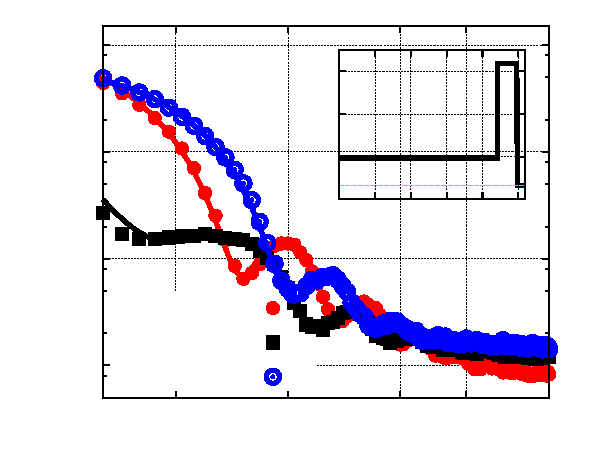
\includegraphics{KiskerSAXSCoreshellFit}}%
    \gplfronttext
  \end{picture}%
\endgroup

		\caption[Core-shell model fit to the PS-COOH particles experimental data.]{The simulated scattering curves from the core-shell model fit at three selected contrasts $\rho_0-\rho_{\text{solv}}$ are shown as lines together with the experimental data points. In the inset, the electron density profile corresponding to the fitted core-shell form factor is displayed.}
		\label{fig:KiskerSAXSCoreshellFit}
\end{figure}

The obtained results are \(R=\left(49.7 \pm 2.8\right) \) nm, \(R_{\text{core}}=\left(44.2 \pm 0.9\right) \) nm, \(\rho_{\text{core}}=\left(339.7 \pm 0.1\right)\) nm\(^{-3}\) and \(\rho_{\text{shell}}=\left(361.9 \pm 2.0\right)\) nm\(^{-3}\), which represent the radial structure of a dense, thin shell surrounding a lighter core, as seen in the inset of figure \ref{fig:KiskerSAXSCoreshellFit}. The resulting average electron density of the particle is \(\rho_{0}=\left(345.9 \pm 1.5\right)\) nm\(^{-3}\) and the polydispersity degree, \(p_d=\left(22.8\pm 6.0\right)\,\%\). The best fitting background corresponds to a value of \( \gamma = 4.3\pm 0.5 \), close to the case \( \gamma = 4 \) originating from large impurities or precipitates \citep{pedersen_determination_1994}. 



The fit uncertainty was calculated with a confidence interval of one standard deviation. 

\textcolor{red}{The main uncertainty contribution is caused by the fitting process with 0.12 nm.}


It is noticeable that the calculated electron density of the core coincides exactly with the theoretical polystyrene electron density, although the electron density of the shell is remarkably lower than the theoretical value of 383.4 nm\(^{-3}\) for PMMA \citep{ballauff_saxs_2001-1}. This might arise from the lower density of the monomers used in the particle synthesis (MAA and MMA), which could have mixed with the styrene monomers resulting in a less dense material than PMMA. This model might present some differences with the real colloid system, as a diffusive interfacial layer could be expected between polymer phases in colloids \citep{dingenouts_interface_1994}, especially for incompatible polymers such as PMMA and PS. On the other hand, the large quantity of scattering curves used for the fitting process and, accordingly, the decreased uncertainty suggests that the chosen sharp core-shell model has a great resemblance to the real particle.

\subsection{Isoscattering point}

Although the first isoscattering point is clearly visible in figure \ref{fig:KiskerContinuousSAXS}, a model-free approach like the isoscattering point requires of a more precise determination of the position and a quantitative evaluation. For this purpose, the relative standard deviation $\sigma_r$ of the 40 measured curves at each \(q\) is calculated according to
\begin{equation}
\sigma_r (q)=\frac{1}{\bar{I}(q)}\sqrt{\frac{\sum^{M}_{i=1} (I_i(q) -\bar{I} (q))^2 }{M-1}} ,
\end{equation}
where \(\bar{I} (q)\) is the mean value of the intensity at \(q\) and \( M \) is the number of scattering curves. This value becomes minimal at an isoscattering point. In order to reduce the influence of outliers, a truncated mean value was utilized, disregarding the 10 $\%$ most dispersed data points. In figure \ref{fig:KiskerIsopoint}, the relative standard deviation is plotted as a function of the momentum transfer \(q\), which shows several distinguishable minima corresponding to isoscattering points.

%\begin{figure}%[htbp]
%	\centering
%		% GNUPLOT: LaTeX picture with Postscript
\begingroup
  \makeatletter
  \providecommand\color[2][]{%
    \GenericError{(gnuplot) \space\space\space\@spaces}{%
      Package color not loaded in conjunction with
      terminal option `colourtext'%
    }{See the gnuplot documentation for explanation.%
    }{Either use 'blacktext' in gnuplot or load the package
      color.sty in LaTeX.}%
    \renewcommand\color[2][]{}%
  }%
  \providecommand\includegraphics[2][]{%
    \GenericError{(gnuplot) \space\space\space\@spaces}{%
      Package graphicx or graphics not loaded%
    }{See the gnuplot documentation for explanation.%
    }{The gnuplot epslatex terminal needs graphicx.sty or graphics.sty.}%
    \renewcommand\includegraphics[2][]{}%
  }%
  \providecommand\rotatebox[2]{#2}%
  \@ifundefined{ifGPcolor}{%
    \newif\ifGPcolor
    \GPcolortrue
  }{}%
  \@ifundefined{ifGPblacktext}{%
    \newif\ifGPblacktext
    \GPblacktextfalse
  }{}%
  % define a \g@addto@macro without @ in the name:
  \let\gplgaddtomacro\g@addto@macro
  % define empty templates for all commands taking text:
  \gdef\gplbacktext{}%
  \gdef\gplfronttext{}%
  \makeatother
  \ifGPblacktext
    % no textcolor at all
    \def\colorrgb#1{}%
    \def\colorgray#1{}%
  \else
    % gray or color?
    \ifGPcolor
      \def\colorrgb#1{\color[rgb]{#1}}%
      \def\colorgray#1{\color[gray]{#1}}%
      \expandafter\def\csname LTw\endcsname{\color{white}}%
      \expandafter\def\csname LTb\endcsname{\color{black}}%
      \expandafter\def\csname LTa\endcsname{\color{black}}%
      \expandafter\def\csname LT0\endcsname{\color[rgb]{1,0,0}}%
      \expandafter\def\csname LT1\endcsname{\color[rgb]{0,1,0}}%
      \expandafter\def\csname LT2\endcsname{\color[rgb]{0,0,1}}%
      \expandafter\def\csname LT3\endcsname{\color[rgb]{1,0,1}}%
      \expandafter\def\csname LT4\endcsname{\color[rgb]{0,1,1}}%
      \expandafter\def\csname LT5\endcsname{\color[rgb]{1,1,0}}%
      \expandafter\def\csname LT6\endcsname{\color[rgb]{0,0,0}}%
      \expandafter\def\csname LT7\endcsname{\color[rgb]{1,0.3,0}}%
      \expandafter\def\csname LT8\endcsname{\color[rgb]{0.5,0.5,0.5}}%
    \else
      % gray
      \def\colorrgb#1{\color{black}}%
      \def\colorgray#1{\color[gray]{#1}}%
      \expandafter\def\csname LTw\endcsname{\color{white}}%
      \expandafter\def\csname LTb\endcsname{\color{black}}%
      \expandafter\def\csname LTa\endcsname{\color{black}}%
      \expandafter\def\csname LT0\endcsname{\color{black}}%
      \expandafter\def\csname LT1\endcsname{\color{black}}%
      \expandafter\def\csname LT2\endcsname{\color{black}}%
      \expandafter\def\csname LT3\endcsname{\color{black}}%
      \expandafter\def\csname LT4\endcsname{\color{black}}%
      \expandafter\def\csname LT5\endcsname{\color{black}}%
      \expandafter\def\csname LT6\endcsname{\color{black}}%
      \expandafter\def\csname LT7\endcsname{\color{black}}%
      \expandafter\def\csname LT8\endcsname{\color{black}}%
    \fi
  \fi
  \setlength{\unitlength}{0.0500bp}%
  \begin{picture}(5668.00,4534.00)%
    \gplgaddtomacro\gplbacktext{%
      \csname LTb\endcsname%
      \put(946,1439){\makebox(0,0)[r]{\strut{} 0.1}}%
      \csname LTb\endcsname%
      \put(946,2291){\makebox(0,0)[r]{\strut{} 0.2}}%
      \csname LTb\endcsname%
      \put(946,3417){\makebox(0,0)[r]{\strut{} 0.5}}%
      \csname LTb\endcsname%
      \put(946,4269){\makebox(0,0)[r]{\strut{} 1}}%
      \csname LTb\endcsname%
      \put(1078,484){\makebox(0,0){\strut{} 0.07}}%
      \csname LTb\endcsname%
      \put(1839,484){\makebox(0,0){\strut{} 0.1}}%
      \csname LTb\endcsname%
      \put(3317,484){\makebox(0,0){\strut{} 0.2}}%
      \csname LTb\endcsname%
      \put(5271,484){\makebox(0,0){\strut{} 0.5}}%
      \put(176,2486){\rotatebox{-270}{\makebox(0,0){\strut{}Rel. Std. Deviation}}}%
      \put(3174,154){\makebox(0,0){\strut{}$q$ / nm$^{-1}$}}%
      \put(1225,1611){\makebox(0,0)[l]{\strut{}$q^{\star}_1$}}%
      \put(2315,1439){\makebox(0,0)[l]{\strut{}$q^{\star}_2$}}%
      \put(3092,1239){\makebox(0,0)[l]{\strut{}$q^{\star}_3$}}%
      \put(4252,1439){\makebox(0,0)[l]{\strut{}$q^{\star}_4$}}%
      \put(4600,1808){\makebox(0,0)[l]{\strut{}$q^{\star}_5$}}%
    }%
    \gplgaddtomacro\gplfronttext{%
    }%
    \gplbacktext
    \put(0,0){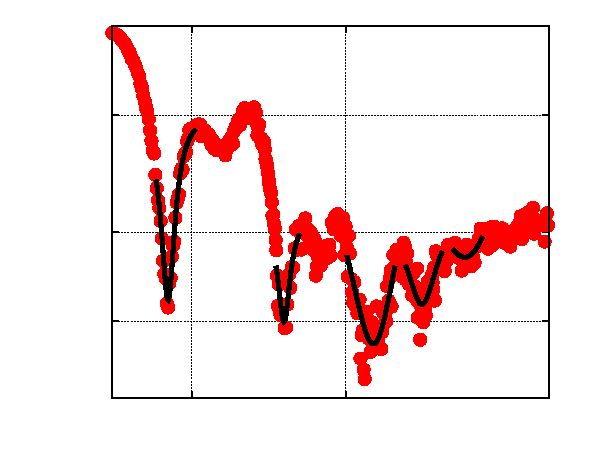
\includegraphics{KiskerIsopoint}}%
    \gplfronttext
  \end{picture}%
\endgroup

%		\caption{Relative standard deviation of the scattering curves as a function of the momentum transfer. The labelled minima correspond to the first five isoscattering point positions calculated by fitting a Lorentzian function (red line).}
%		\label{fig:KiskerIsopoint}
%\end{figure}

%\begin{table}
%\caption{Experimentally determined position of the first five isoscattering points and the corresponding external particle radius $R$.}
%\begin{tabular}{l|cc}
% & \( q^{\star} \) (nm\(^{-1}\))    &  \(R\) (nm) \\
%\hline
% \(q^{\star}_1\) &  0.0900 & 49.9 \\
% \(q^{\star}_2\) &  0.1516 & 51.0  \\
% \(q^{\star}_3\) &  0.2267 & 48.1   \\
% \(q^{\star}_4\) &  0.2822 & 49.9    \\
% \(q^{\star}_5\) &  0.3421 & 50.3     \\
%\end{tabular}
%\label{tab:isopoint_Kisker}
%\end{table}

\begin{figure*}
    \centering
    \subfloat[Relative standard deviation]{
        \resizebox{0.44\linewidth}{!}{\figfont{13pt}% GNUPLOT: LaTeX picture with Postscript
\begingroup
  \makeatletter
  \providecommand\color[2][]{%
    \GenericError{(gnuplot) \space\space\space\@spaces}{%
      Package color not loaded in conjunction with
      terminal option `colourtext'%
    }{See the gnuplot documentation for explanation.%
    }{Either use 'blacktext' in gnuplot or load the package
      color.sty in LaTeX.}%
    \renewcommand\color[2][]{}%
  }%
  \providecommand\includegraphics[2][]{%
    \GenericError{(gnuplot) \space\space\space\@spaces}{%
      Package graphicx or graphics not loaded%
    }{See the gnuplot documentation for explanation.%
    }{The gnuplot epslatex terminal needs graphicx.sty or graphics.sty.}%
    \renewcommand\includegraphics[2][]{}%
  }%
  \providecommand\rotatebox[2]{#2}%
  \@ifundefined{ifGPcolor}{%
    \newif\ifGPcolor
    \GPcolortrue
  }{}%
  \@ifundefined{ifGPblacktext}{%
    \newif\ifGPblacktext
    \GPblacktextfalse
  }{}%
  % define a \g@addto@macro without @ in the name:
  \let\gplgaddtomacro\g@addto@macro
  % define empty templates for all commands taking text:
  \gdef\gplbacktext{}%
  \gdef\gplfronttext{}%
  \makeatother
  \ifGPblacktext
    % no textcolor at all
    \def\colorrgb#1{}%
    \def\colorgray#1{}%
  \else
    % gray or color?
    \ifGPcolor
      \def\colorrgb#1{\color[rgb]{#1}}%
      \def\colorgray#1{\color[gray]{#1}}%
      \expandafter\def\csname LTw\endcsname{\color{white}}%
      \expandafter\def\csname LTb\endcsname{\color{black}}%
      \expandafter\def\csname LTa\endcsname{\color{black}}%
      \expandafter\def\csname LT0\endcsname{\color[rgb]{1,0,0}}%
      \expandafter\def\csname LT1\endcsname{\color[rgb]{0,1,0}}%
      \expandafter\def\csname LT2\endcsname{\color[rgb]{0,0,1}}%
      \expandafter\def\csname LT3\endcsname{\color[rgb]{1,0,1}}%
      \expandafter\def\csname LT4\endcsname{\color[rgb]{0,1,1}}%
      \expandafter\def\csname LT5\endcsname{\color[rgb]{1,1,0}}%
      \expandafter\def\csname LT6\endcsname{\color[rgb]{0,0,0}}%
      \expandafter\def\csname LT7\endcsname{\color[rgb]{1,0.3,0}}%
      \expandafter\def\csname LT8\endcsname{\color[rgb]{0.5,0.5,0.5}}%
    \else
      % gray
      \def\colorrgb#1{\color{black}}%
      \def\colorgray#1{\color[gray]{#1}}%
      \expandafter\def\csname LTw\endcsname{\color{white}}%
      \expandafter\def\csname LTb\endcsname{\color{black}}%
      \expandafter\def\csname LTa\endcsname{\color{black}}%
      \expandafter\def\csname LT0\endcsname{\color{black}}%
      \expandafter\def\csname LT1\endcsname{\color{black}}%
      \expandafter\def\csname LT2\endcsname{\color{black}}%
      \expandafter\def\csname LT3\endcsname{\color{black}}%
      \expandafter\def\csname LT4\endcsname{\color{black}}%
      \expandafter\def\csname LT5\endcsname{\color{black}}%
      \expandafter\def\csname LT6\endcsname{\color{black}}%
      \expandafter\def\csname LT7\endcsname{\color{black}}%
      \expandafter\def\csname LT8\endcsname{\color{black}}%
    \fi
  \fi
  \setlength{\unitlength}{0.0500bp}%
  \begin{picture}(5668.00,4534.00)%
    \gplgaddtomacro\gplbacktext{%
      \csname LTb\endcsname%
      \put(946,1439){\makebox(0,0)[r]{\strut{} 0.1}}%
      \csname LTb\endcsname%
      \put(946,2291){\makebox(0,0)[r]{\strut{} 0.2}}%
      \csname LTb\endcsname%
      \put(946,3417){\makebox(0,0)[r]{\strut{} 0.5}}%
      \csname LTb\endcsname%
      \put(946,4269){\makebox(0,0)[r]{\strut{} 1}}%
      \csname LTb\endcsname%
      \put(1078,484){\makebox(0,0){\strut{} 0.07}}%
      \csname LTb\endcsname%
      \put(1839,484){\makebox(0,0){\strut{} 0.1}}%
      \csname LTb\endcsname%
      \put(3317,484){\makebox(0,0){\strut{} 0.2}}%
      \csname LTb\endcsname%
      \put(5271,484){\makebox(0,0){\strut{} 0.5}}%
      \put(176,2486){\rotatebox{-270}{\makebox(0,0){\strut{}Rel. Std. Deviation}}}%
      \put(3174,154){\makebox(0,0){\strut{}$q$ / nm$^{-1}$}}%
      \put(1225,1611){\makebox(0,0)[l]{\strut{}$q^{\star}_1$}}%
      \put(2315,1439){\makebox(0,0)[l]{\strut{}$q^{\star}_2$}}%
      \put(3092,1239){\makebox(0,0)[l]{\strut{}$q^{\star}_3$}}%
      \put(4252,1439){\makebox(0,0)[l]{\strut{}$q^{\star}_4$}}%
      \put(4600,1808){\makebox(0,0)[l]{\strut{}$q^{\star}_5$}}%
    }%
    \gplgaddtomacro\gplfronttext{%
    }%
    \gplbacktext
    \put(0,0){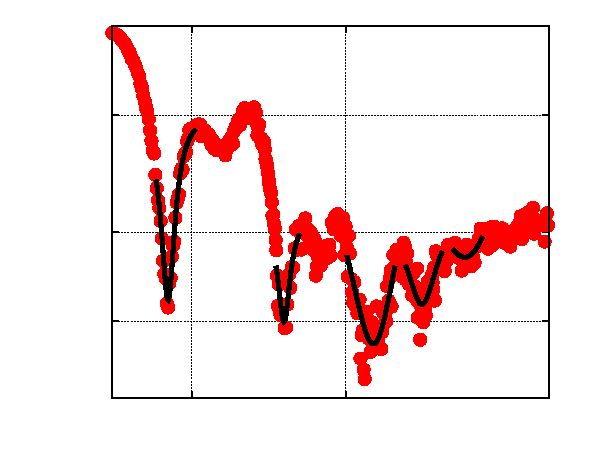
\includegraphics{KiskerIsopoint}}%
    \gplfronttext
  \end{picture}%
\endgroup
}
        \label{fig:KiskerIsopoint}
    }
    \subfloat[Isoscattering point positions]{
	\renewcommand{\arraystretch}{1.3}
        \begin{tabular}[b]{l|ccc}
         & \( q^{\star} \) (nm\(^{-1}\))    &  \(R\) (nm)    &  \textcolor{red}{\(\delta R\) (nm)} \\
        \hline
         \(q^{\star}_1\) &  0.0900 & 49.9 & 5.5 \\
         \(q^{\star}_2\) &  0.1516 & 51.0 & 4.6  \\
         \(q^{\star}_3\) &  0.2267 & 48.1 & 3.8   \\
         \(q^{\star}_4\) &  0.2822 & 49.9 & 5.0    \\
         \(q^{\star}_5\) &  0.3421 & 50.3 & 7.5     \\
         
         \hline
         
         \textcolor{red}{mean} & \textcolor{red}{XXX}  & \textcolor{red}{49.7} & \textcolor{red}{???}     \\
         \end{tabular}
         \label{tab:isopoint_Kisker}
    }
\caption[Isoscattering points of the PS-COOH particles.]{Isoscattering points of the PS-COOH particles: a) Relative standard deviation of the scattering curves as a function of the momentum transfer. The labelled minima correspond to the first five isoscattering point positions calculated by fitting a Lorentzian function (black line). b) Experimentally determined position of the first five isoscattering points and the corresponding external particle radius $R$.}    
\end{figure*}

A precise determination of the isoscattering point positions is performed by fitting Lorentzian functions to the minima in the relative standard deviation plot, which allows the calculation of the model-free external radius of the particle by means of equation \eqref{eq:isoscattering}. The results are presented in table \ref{tab:isopoint_Kisker}. The obtained particle radii vary in the range from \(48.1\) nm to \(51.0\) nm, although as predicted by \cite{kawaguchi_isoscattering_1992} for a polydisperse system, the isoscattering points get smeared out for larger \( q \)-values and the precision decreases, simultaneously with the increase of the solvent background at higher \(q\)-values. This can be directly observed in the quality of the experimental data, as the first two minima are clearly pronounced, while the subsequent minima appear smeared out. For instance, the isoscattering point \(q^{\star}_5\) is already too weak for an accurate evaluation and the third minimum shows two remarkably close smaller minima which might affect the shape of the function. Therefore, \(q^{\star}_1\) and \(q^{\star}_2\) yield the most reliable values for evaluating the external radius of the particles, although all results are presented in table \ref{tab:isopoint_Kisker}. The value derived from the isoscattering points \(R=50.5\) nm differs by only 1.6 $\%$ from the radius calculated from the model fit in the previous section.

Due to the ambiguous definition of the isoscattering point diffuseness, a quantitative determination of the polydispersity of the suspended nanoparticles by means of the Lorentzian profile is rather challenging. Nevertheless, the narrow size distribution of the sample becomes clear by comparing the relative standard deviation values of the observed minima in figure \ref{fig:KiskerIsopoint} with a simulation using the structural parameters obtained in section \ref{sec:coreshell_fit}. The value \( \sigma_r(q^{\star}_1)=0.11 \) corresponds to a calculated ensemble polydispersity of 24 $\%$. This value serves as an upper \( p_d \) limit due to the possible overestimation caused by the scattering contribution of the suspending medium.


\subsection{Guinier region}
\label{sec:guinier_analysis}
By analysing the low \(q \)-region of the scattering curves, the so-called Guinier region, two important parameters can be obtained: the radius of gyration \(R_g\) and the intensity at zero angle \(I(0)\). According to \cite{feigin_structure_1987}, the fit of equation \eqref{eq:guinier} to the Guinier region is mainly valid up to \( qR_g<1.3 \). In this restricted \(q\)-range, too few data points are available for a reliable data analysis. Therefore, an extrapolation using the spherical form factor \( F_{\text{sph}}(q,R) \) over the range available before the first minimum has been employed instead to obtain \(R_g\) and \(I(0)\). This arises as a good choice because the Guinier approximation overestimates the values of the zero-angle intensity due to its limitation to monodisperse systems \citep{feigin_structure_1987}, as observed in figure \ref{fig:KiskerIntensityComparison}. On the other hand, a more primitive approach, e.g. the intensity of the lowest accessible $q$-value ($q_{\text{min}}=0.03$ nm$^{-1}$), underestimates the $I(0)$ values, because it neglects the extrapolation to $q\rightarrow0$, as shown also in figure \ref{fig:KiskerIntensityComparison}.

\begin{figure}%[htbp]
	\centering
		% GNUPLOT: LaTeX picture with Postscript
\begingroup
  \makeatletter
  \providecommand\color[2][]{%
    \GenericError{(gnuplot) \space\space\space\@spaces}{%
      Package color not loaded in conjunction with
      terminal option `colourtext'%
    }{See the gnuplot documentation for explanation.%
    }{Either use 'blacktext' in gnuplot or load the package
      color.sty in LaTeX.}%
    \renewcommand\color[2][]{}%
  }%
  \providecommand\includegraphics[2][]{%
    \GenericError{(gnuplot) \space\space\space\@spaces}{%
      Package graphicx or graphics not loaded%
    }{See the gnuplot documentation for explanation.%
    }{The gnuplot epslatex terminal needs graphicx.sty or graphics.sty.}%
    \renewcommand\includegraphics[2][]{}%
  }%
  \providecommand\rotatebox[2]{#2}%
  \@ifundefined{ifGPcolor}{%
    \newif\ifGPcolor
    \GPcolortrue
  }{}%
  \@ifundefined{ifGPblacktext}{%
    \newif\ifGPblacktext
    \GPblacktextfalse
  }{}%
  % define a \g@addto@macro without @ in the name:
  \let\gplgaddtomacro\g@addto@macro
  % define empty templates for all commands taking text:
  \gdef\gplbacktext{}%
  \gdef\gplfronttext{}%
  \makeatother
  \ifGPblacktext
    % no textcolor at all
    \def\colorrgb#1{}%
    \def\colorgray#1{}%
  \else
    % gray or color?
    \ifGPcolor
      \def\colorrgb#1{\color[rgb]{#1}}%
      \def\colorgray#1{\color[gray]{#1}}%
      \expandafter\def\csname LTw\endcsname{\color{white}}%
      \expandafter\def\csname LTb\endcsname{\color{black}}%
      \expandafter\def\csname LTa\endcsname{\color{black}}%
      \expandafter\def\csname LT0\endcsname{\color[rgb]{1,0,0}}%
      \expandafter\def\csname LT1\endcsname{\color[rgb]{0,1,0}}%
      \expandafter\def\csname LT2\endcsname{\color[rgb]{0,0,1}}%
      \expandafter\def\csname LT3\endcsname{\color[rgb]{1,0,1}}%
      \expandafter\def\csname LT4\endcsname{\color[rgb]{0,1,1}}%
      \expandafter\def\csname LT5\endcsname{\color[rgb]{1,1,0}}%
      \expandafter\def\csname LT6\endcsname{\color[rgb]{0,0,0}}%
      \expandafter\def\csname LT7\endcsname{\color[rgb]{1,0.3,0}}%
      \expandafter\def\csname LT8\endcsname{\color[rgb]{0.5,0.5,0.5}}%
    \else
      % gray
      \def\colorrgb#1{\color{black}}%
      \def\colorgray#1{\color[gray]{#1}}%
      \expandafter\def\csname LTw\endcsname{\color{white}}%
      \expandafter\def\csname LTb\endcsname{\color{black}}%
      \expandafter\def\csname LTa\endcsname{\color{black}}%
      \expandafter\def\csname LT0\endcsname{\color{black}}%
      \expandafter\def\csname LT1\endcsname{\color{black}}%
      \expandafter\def\csname LT2\endcsname{\color{black}}%
      \expandafter\def\csname LT3\endcsname{\color{black}}%
      \expandafter\def\csname LT4\endcsname{\color{black}}%
      \expandafter\def\csname LT5\endcsname{\color{black}}%
      \expandafter\def\csname LT6\endcsname{\color{black}}%
      \expandafter\def\csname LT7\endcsname{\color{black}}%
      \expandafter\def\csname LT8\endcsname{\color{black}}%
    \fi
  \fi
    \setlength{\unitlength}{0.0500bp}%
    \ifx\gptboxheight\undefined%
      \newlength{\gptboxheight}%
      \newlength{\gptboxwidth}%
      \newsavebox{\gptboxtext}%
    \fi%
    \setlength{\fboxrule}{0.5pt}%
    \setlength{\fboxsep}{1pt}%
\begin{picture}(5668.00,4534.00)%
    \gplgaddtomacro\gplbacktext{%
      \csname LTb\endcsname%
      \put(814,839){\makebox(0,0)[r]{\strut{}$-40$}}%
      \csname LTb\endcsname%
      \put(814,1511){\makebox(0,0)[r]{\strut{}$-20$}}%
      \csname LTb\endcsname%
      \put(814,2184){\makebox(0,0)[r]{\strut{}$0$}}%
      \csname LTb\endcsname%
      \put(814,2856){\makebox(0,0)[r]{\strut{}$20$}}%
      \csname LTb\endcsname%
      \put(814,3529){\makebox(0,0)[r]{\strut{}$40$}}%
      \csname LTb\endcsname%
      \put(814,4202){\makebox(0,0)[r]{\strut{}$60$}}%
      \csname LTb\endcsname%
      \put(1250,484){\makebox(0,0){\strut{}$335$}}%
      \csname LTb\endcsname%
      \put(2008,484){\makebox(0,0){\strut{}$340$}}%
      \csname LTb\endcsname%
      \put(2767,484){\makebox(0,0){\strut{}$345$}}%
      \csname LTb\endcsname%
      \put(3526,484){\makebox(0,0){\strut{}$350$}}%
      \csname LTb\endcsname%
      \put(4285,484){\makebox(0,0){\strut{}$355$}}%
      \csname LTb\endcsname%
      \put(5043,484){\makebox(0,0){\strut{}$360$}}%
    }%
    \gplgaddtomacro\gplfronttext{%
      \csname LTb\endcsname%
      \put(176,2486){\rotatebox{-270}{\makebox(0,0){\strut{}Deviation from $I(0)$ / $\%$}}}%
      \put(3108,154){\makebox(0,0){\strut{}Solvent electron density / nm$^{-3}$}}%
      \csname LTb\endcsname%
      \put(4548,4041){\makebox(0,0)[r]{\strut{}\smaller Guinier approximation}}%
      \csname LTb\endcsname%
      \put(4548,3711){\makebox(0,0)[r]{\strut{}\smaller Lowest available $q$}}%
    }%
    \gplbacktext
    \put(0,0){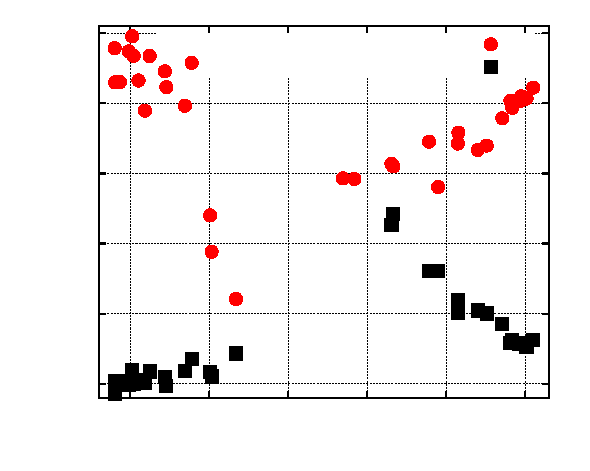
\includegraphics{KiskerIntensityComparison}}%
    \gplfronttext
  \end{picture}%
\endgroup

		\caption[Deviation from the $I(0)$ used in the evaluation of the PS-COOH particles experimental data.]{Deviation from the $I(0)$ values used in the data evaluation: The Guinier approximation overestimates the experimental values, while the intensity at $q=0.03$ nm$^{-1}$ underestimates the zero-angle intensity.}
		\label{fig:KiskerIntensityComparison}
\end{figure}

As described in section \ref{sec:TheoryGuinier}, the radius of gyration of a heterogeneous particle in a contrast variation experiment should behave according to equation \eqref{eq:gyration}. In figure \ref{fig:KiskerGuinierRadius}, the experimental squared radius of gyration is displayed as a function of the suspending medium electron density. The best fit to the measured data with values \(\rho_0=343.7\) nm\(^{-3}\), \( \tilde R_{g,c}=39.0\) nm, \(\tilde \alpha=4470\) nm\(^{-1}\) and \(\tilde\beta=0\) nm\(^{-4}\) is shown by the solid line. 

\begin{figure}%[htbp]
	\centering
		% GNUPLOT: LaTeX picture with Postscript
\begingroup
  \makeatletter
  \providecommand\color[2][]{%
    \GenericError{(gnuplot) \space\space\space\@spaces}{%
      Package color not loaded in conjunction with
      terminal option `colourtext'%
    }{See the gnuplot documentation for explanation.%
    }{Either use 'blacktext' in gnuplot or load the package
      color.sty in LaTeX.}%
    \renewcommand\color[2][]{}%
  }%
  \providecommand\includegraphics[2][]{%
    \GenericError{(gnuplot) \space\space\space\@spaces}{%
      Package graphicx or graphics not loaded%
    }{See the gnuplot documentation for explanation.%
    }{The gnuplot epslatex terminal needs graphicx.sty or graphics.sty.}%
    \renewcommand\includegraphics[2][]{}%
  }%
  \providecommand\rotatebox[2]{#2}%
  \@ifundefined{ifGPcolor}{%
    \newif\ifGPcolor
    \GPcolortrue
  }{}%
  \@ifundefined{ifGPblacktext}{%
    \newif\ifGPblacktext
    \GPblacktextfalse
  }{}%
  % define a \g@addto@macro without @ in the name:
  \let\gplgaddtomacro\g@addto@macro
  % define empty templates for all commands taking text:
  \gdef\gplbacktext{}%
  \gdef\gplfronttext{}%
  \makeatother
  \ifGPblacktext
    % no textcolor at all
    \def\colorrgb#1{}%
    \def\colorgray#1{}%
  \else
    % gray or color?
    \ifGPcolor
      \def\colorrgb#1{\color[rgb]{#1}}%
      \def\colorgray#1{\color[gray]{#1}}%
      \expandafter\def\csname LTw\endcsname{\color{white}}%
      \expandafter\def\csname LTb\endcsname{\color{black}}%
      \expandafter\def\csname LTa\endcsname{\color{black}}%
      \expandafter\def\csname LT0\endcsname{\color[rgb]{1,0,0}}%
      \expandafter\def\csname LT1\endcsname{\color[rgb]{0,1,0}}%
      \expandafter\def\csname LT2\endcsname{\color[rgb]{0,0,1}}%
      \expandafter\def\csname LT3\endcsname{\color[rgb]{1,0,1}}%
      \expandafter\def\csname LT4\endcsname{\color[rgb]{0,1,1}}%
      \expandafter\def\csname LT5\endcsname{\color[rgb]{1,1,0}}%
      \expandafter\def\csname LT6\endcsname{\color[rgb]{0,0,0}}%
      \expandafter\def\csname LT7\endcsname{\color[rgb]{1,0.3,0}}%
      \expandafter\def\csname LT8\endcsname{\color[rgb]{0.5,0.5,0.5}}%
    \else
      % gray
      \def\colorrgb#1{\color{black}}%
      \def\colorgray#1{\color[gray]{#1}}%
      \expandafter\def\csname LTw\endcsname{\color{white}}%
      \expandafter\def\csname LTb\endcsname{\color{black}}%
      \expandafter\def\csname LTa\endcsname{\color{black}}%
      \expandafter\def\csname LT0\endcsname{\color{black}}%
      \expandafter\def\csname LT1\endcsname{\color{black}}%
      \expandafter\def\csname LT2\endcsname{\color{black}}%
      \expandafter\def\csname LT3\endcsname{\color{black}}%
      \expandafter\def\csname LT4\endcsname{\color{black}}%
      \expandafter\def\csname LT5\endcsname{\color{black}}%
      \expandafter\def\csname LT6\endcsname{\color{black}}%
      \expandafter\def\csname LT7\endcsname{\color{black}}%
      \expandafter\def\csname LT8\endcsname{\color{black}}%
    \fi
  \fi
  \setlength{\unitlength}{0.0500bp}%
  \begin{picture}(5668.00,4534.00)%
    \gplgaddtomacro\gplbacktext{%
      \csname LTb\endcsname%
      \put(1078,704){\makebox(0,0)[r]{\strut{} 500}}%
      \csname LTb\endcsname%
      \put(1078,1341){\makebox(0,0)[r]{\strut{} 1000}}%
      \csname LTb\endcsname%
      \put(1078,1977){\makebox(0,0)[r]{\strut{} 1500}}%
      \csname LTb\endcsname%
      \put(1078,2614){\makebox(0,0)[r]{\strut{} 2000}}%
      \csname LTb\endcsname%
      \put(1078,3250){\makebox(0,0)[r]{\strut{} 2500}}%
      \csname LTb\endcsname%
      \put(1078,3887){\makebox(0,0)[r]{\strut{} 3000}}%
      \csname LTb\endcsname%
      \put(1210,484){\makebox(0,0){\strut{} 330}}%
      \csname LTb\endcsname%
      \put(1718,484){\makebox(0,0){\strut{} 335}}%
      \csname LTb\endcsname%
      \put(2225,484){\makebox(0,0){\strut{} 340}}%
      \csname LTb\endcsname%
      \put(2733,484){\makebox(0,0){\strut{} 345}}%
      \csname LTb\endcsname%
      \put(3241,484){\makebox(0,0){\strut{} 350}}%
      \csname LTb\endcsname%
      \put(3748,484){\makebox(0,0){\strut{} 355}}%
      \csname LTb\endcsname%
      \put(4256,484){\makebox(0,0){\strut{} 360}}%
      \csname LTb\endcsname%
      \put(4763,484){\makebox(0,0){\strut{} 365}}%
      \csname LTb\endcsname%
      \put(5271,484){\makebox(0,0){\strut{} 370}}%
      \put(176,2486){\rotatebox{-270}{\makebox(0,0){\strut{}$R_g^2$ / nm$^2$}}}%
      \put(3240,154){\makebox(0,0){\strut{}Solvent electron density / nm$^{-3}$}}%
      \put(2733,3887){\makebox(0,0)[l]{\strut{}$\rho_0$}}%
      \put(4763,2232){\makebox(0,0)[l]{\strut{}$\tilde R^2_{g,c}$}}%
    }%
    \gplgaddtomacro\gplfronttext{%
    }%
    \gplbacktext
    \put(0,0){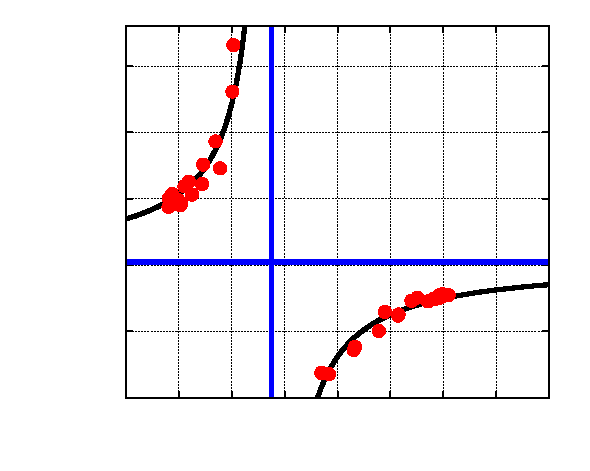
\includegraphics{KiskerGuinierRadius}}%
    \gplfronttext
  \end{picture}%
\endgroup

		\caption[Radius of gyration of the PS-COOH particles.]{Experimental squared radius of gyration as a function of the solvent electron density. Equation \eqref{eq:gyration} is fitted to the data and shown as a thick line. The vertical and horizontal asymptotes correspond to $\rho_0$ and $\tilde R^2_{g,c}$ respectively.}
		\label{fig:KiskerGuinierRadius}
\end{figure}

The positive value of \(\tilde\alpha\) validates the hypothesis that a more dense polymer like PMMA surrounds a lighter core (PS) \citep{stuhrmann_small-angle_2008}. The calculated average electron density of the particle \(\rho_0\) suggests a very thin layer of PMMA shell around the PS core, due to the proximity of its value to the polystyrene electron density (339.7 nm\(^{-3}\) ). The value of \( \tilde\beta=0\) proves a concentric model, where core and shell share the same centre. Using the same polydispersity value of 22.8 $\%$ obtained in the fitting process, the value for the particle shape radius of gyration results in \(R_{g,c}=36.9\) nm and the external radius of the particle can be calculated assuming the particle as a spherical object. This calculation gives \( R=47.6\) nm, which is only 2.1 nm smaller than the calculated external radius \(R=49.7\) nm, though it might be underestimated due to the choice of a possibly inflated polydispersity. 

\subsubsection{Average electron density}
Using the same set of 40 scattering curves, the behaviour of the zero-angle intensity under the contrast variation is also investigated by fitting equation \eqref{eq:I0} to the experimental \(I(0)\), as depicted in figure \ref{fig:KiskerIntensityParabola}. A minimum in the curve is observed at \(\rho_{\text{solv}}=346.0\) nm\(^{-3}\), which corresponds to the value of the average electron density of the particle. This value is in very good agreement with the result obtained by fitting the core-shell form factor. It is also noticeable that the minimum intensity is approximately 0, which means that the effective average density of the ensemble is equal to the average density of the particle \citep{avdeev_contrast_2007}. This result further legitimates the assumption made previously in section \ref{sec:KiskerResults} about the PS-COOH particles that the ratio between the particle components' volumes is constant independent of the polydispersity and hence \(  \tilde \rho_0 = \rho_0  \), i.e. the average density of the particle is not altered by the size polydispersity.

\begin{figure}%[htbp]
	\centering
		% GNUPLOT: LaTeX picture with Postscript
\begingroup
  \makeatletter
  \providecommand\color[2][]{%
    \GenericError{(gnuplot) \space\space\space\@spaces}{%
      Package color not loaded in conjunction with
      terminal option `colourtext'%
    }{See the gnuplot documentation for explanation.%
    }{Either use 'blacktext' in gnuplot or load the package
      color.sty in LaTeX.}%
    \renewcommand\color[2][]{}%
  }%
  \providecommand\includegraphics[2][]{%
    \GenericError{(gnuplot) \space\space\space\@spaces}{%
      Package graphicx or graphics not loaded%
    }{See the gnuplot documentation for explanation.%
    }{The gnuplot epslatex terminal needs graphicx.sty or graphics.sty.}%
    \renewcommand\includegraphics[2][]{}%
  }%
  \providecommand\rotatebox[2]{#2}%
  \@ifundefined{ifGPcolor}{%
    \newif\ifGPcolor
    \GPcolortrue
  }{}%
  \@ifundefined{ifGPblacktext}{%
    \newif\ifGPblacktext
    \GPblacktextfalse
  }{}%
  % define a \g@addto@macro without @ in the name:
  \let\gplgaddtomacro\g@addto@macro
  % define empty templates for all commands taking text:
  \gdef\gplbacktext{}%
  \gdef\gplfronttext{}%
  \makeatother
  \ifGPblacktext
    % no textcolor at all
    \def\colorrgb#1{}%
    \def\colorgray#1{}%
  \else
    % gray or color?
    \ifGPcolor
      \def\colorrgb#1{\color[rgb]{#1}}%
      \def\colorgray#1{\color[gray]{#1}}%
      \expandafter\def\csname LTw\endcsname{\color{white}}%
      \expandafter\def\csname LTb\endcsname{\color{black}}%
      \expandafter\def\csname LTa\endcsname{\color{black}}%
      \expandafter\def\csname LT0\endcsname{\color[rgb]{1,0,0}}%
      \expandafter\def\csname LT1\endcsname{\color[rgb]{0,1,0}}%
      \expandafter\def\csname LT2\endcsname{\color[rgb]{0,0,1}}%
      \expandafter\def\csname LT3\endcsname{\color[rgb]{1,0,1}}%
      \expandafter\def\csname LT4\endcsname{\color[rgb]{0,1,1}}%
      \expandafter\def\csname LT5\endcsname{\color[rgb]{1,1,0}}%
      \expandafter\def\csname LT6\endcsname{\color[rgb]{0,0,0}}%
      \expandafter\def\csname LT7\endcsname{\color[rgb]{1,0.3,0}}%
      \expandafter\def\csname LT8\endcsname{\color[rgb]{0.5,0.5,0.5}}%
    \else
      % gray
      \def\colorrgb#1{\color{black}}%
      \def\colorgray#1{\color[gray]{#1}}%
      \expandafter\def\csname LTw\endcsname{\color{white}}%
      \expandafter\def\csname LTb\endcsname{\color{black}}%
      \expandafter\def\csname LTa\endcsname{\color{black}}%
      \expandafter\def\csname LT0\endcsname{\color{black}}%
      \expandafter\def\csname LT1\endcsname{\color{black}}%
      \expandafter\def\csname LT2\endcsname{\color{black}}%
      \expandafter\def\csname LT3\endcsname{\color{black}}%
      \expandafter\def\csname LT4\endcsname{\color{black}}%
      \expandafter\def\csname LT5\endcsname{\color{black}}%
      \expandafter\def\csname LT6\endcsname{\color{black}}%
      \expandafter\def\csname LT7\endcsname{\color{black}}%
      \expandafter\def\csname LT8\endcsname{\color{black}}%
    \fi
  \fi
  \setlength{\unitlength}{0.0500bp}%
  \begin{picture}(5668.00,4534.00)%
    \gplgaddtomacro\gplbacktext{%
      \csname LTb\endcsname%
      \put(946,841){\makebox(0,0)[r]{\strut{} 0}}%
      \csname LTb\endcsname%
      \put(946,1298){\makebox(0,0)[r]{\strut{} 0.2}}%
      \csname LTb\endcsname%
      \put(946,1755){\makebox(0,0)[r]{\strut{} 0.4}}%
      \csname LTb\endcsname%
      \put(946,2212){\makebox(0,0)[r]{\strut{} 0.6}}%
      \csname LTb\endcsname%
      \put(946,2669){\makebox(0,0)[r]{\strut{} 0.8}}%
      \csname LTb\endcsname%
      \put(946,3126){\makebox(0,0)[r]{\strut{} 1}}%
      \csname LTb\endcsname%
      \put(946,3583){\makebox(0,0)[r]{\strut{} 1.2}}%
      \csname LTb\endcsname%
      \put(946,4040){\makebox(0,0)[r]{\strut{} 1.4}}%
      \csname LTb\endcsname%
      \put(1378,484){\makebox(0,0){\strut{} 335}}%
      \csname LTb\endcsname%
      \put(2126,484){\makebox(0,0){\strut{} 340}}%
      \csname LTb\endcsname%
      \put(2875,484){\makebox(0,0){\strut{} 345}}%
      \csname LTb\endcsname%
      \put(3624,484){\makebox(0,0){\strut{} 350}}%
      \csname LTb\endcsname%
      \put(4373,484){\makebox(0,0){\strut{} 355}}%
      \csname LTb\endcsname%
      \put(5121,484){\makebox(0,0){\strut{} 360}}%
      \put(176,2486){\rotatebox{-270}{\makebox(0,0){\strut{}$I(0)$ / a.u.}}}%
      \put(3174,154){\makebox(0,0){\strut{}Solvent electron density / nm$^{-3}$}}%
    }%
    \gplgaddtomacro\gplfronttext{%
    }%
    \gplbacktext
    \put(0,0){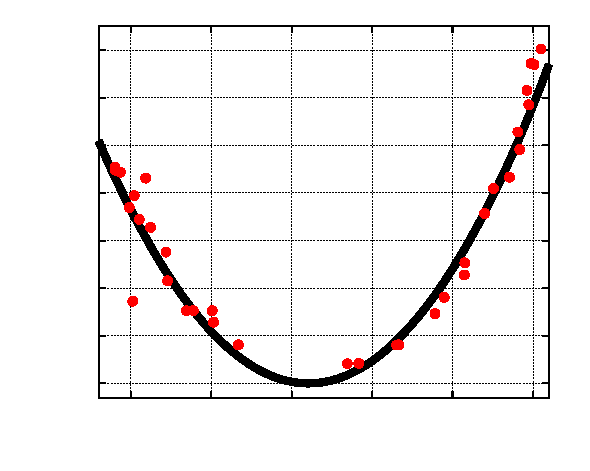
\includegraphics{KiskerIntensityParabola}}%
    \gplfronttext
  \end{picture}%
\endgroup

		\caption[Zero-angle intensity of the PS-COOH particles.]{Experimental zero-angle intensity as a function of the solvent electron density. The function corresponding to equation \eqref{eq:I0} is fitted to the data and shown as a thick line. The minimum in the parabola corresponds to $\rho_{\text{solv}}=\rho_0$.}
		\label{fig:KiskerIntensityParabola}
\end{figure}

\subsection{Consistency of the results}
Table \ref{tab:comparison_results_Kisker} summarizes the results of all three presented methods. From the first two isoscattering points, values for the external radius and an upper bound to the polydispersity degree have been derived. Focusing on the Guinier region of the scattering curves, a value for the average electron density of the particles is found using the radius of gyration as well as the zero-angle intensity, the values of which differ by 2.3 nm\(^{-3}\). By fitting a core-shell model, an external radius of \(R=49.7\) nm and an average electron density \(\rho_0=345.9\) nm\(^{-3}\) have been obtained, which are in considerable agreement with the previous results, i.e., the values determined by the other methods are included in their confidence ranges, except for the \(\rho_0\) calculated with the radii of gyration.

From these results, it is evident that the radius of gyration interpretation produces the most deviant values. This might be founded in the complicated function fitted to the data and the reduced availability of $q$-range employed to obtain \( R_g \). The resulting polydispersity degree of the measured particles from the model fit is in agreement with the upper limit obtained with the radii of gyration. Nevertheless the polydispersity is the parameter determined with the largest uncertainty in the fitting process and therefore this result must be considered with care.

It can be concluded that the different approaches show consistent and complementary results about the size distribution of nanoparticles with radial inner structure, especially for the external radius of the particle and its average electron density. A precise value for the polydispersity degree could not be obtained as explained previously, although a credible upper limit to the polydispersity degree of 24 $\%$ could be given.

\begin{table*}
\caption[Comparison of the results obtained by different evaluation approaches to contrast variation SAXS data.]{Comparison of the results obtained by the different approaches presented in section \ref{sec:KiskerResultsEvaluation} to evaluate contrast variation SAXS data.}
\begin{tabular}{l|ccc}
 & \( R\) (nm)    & \(\rho_0\) (nm\(^{-3}\)) & \(p_d\) (\(\%\))\\
\hline
 Core-shell fitting &  49.7\(\pm 2.8\)   &     345.9\(\pm 1.5\)      & 22.8\(\pm 6.0\) \\
 Isoscattering point &  \textcolor{red}{50.5\(\pm 3.6\)*} &     -          & $<24$  \\
 Radius of gyration &  47.6**      &     343.7      & -    \\
 Zero-angle intensity &  -    &     \textcolor{red}{346.0\(\pm 1.5\)}      & -    \\ \hline
\multicolumn{4}{r}{*Mean value of \(q^{\star}_1\) and \(q^{\star}_2\)}\\  
\multicolumn{4}{r}{**Using the polydispersity degree from the core-shell model fitting}\\ 
\end{tabular}
\label{tab:comparison_results_Kisker}
\end{table*}

\section{Applicability and comparison with other contrast variation approaches}
\label{sec:applicability}

The accessible electron density range defines the possible applications of the proposed technique and is consequently the most decisive factor to choose the contrast agent. With saccharides like sucrose or fructose, high concentrated mixtures with low viscosity can be achieved, reaching electron densities up to 400 nm$^{-3}$. Sugars are suitable for contrast variation experiments with bio-materials and polymeric nanoparticles, whose densities typically range between 0.9 and 1.4 g cm$^{-3}$ (from 300 to 450 nm$^{-3}$). On the other hand, contrast agents like ethanol can reduce the electron density of the suspending medium until 270 nm$^{-3}$ and, besides, is perfectly miscible with water. A wide variety of biological particles exist within the available density range achieved between ethanol and sugar.

More dense solutions prepared with heavy salts (e.g. sodium polytungstate (SPT)) could be an alternative for heavier particles e.g. silica, similarly to the application in sink-float analysis and density gradient centrifugation \citep{rhodes_fine_1991,mitchell_setup_2010}. Nevertheless, the salt can compromise the stability of the particles inducing aggregation and lead to more complicated handling of the sample due to a decreased diffusion timescale. The chemical stability of the suspension is a crucial parameter that depends specifically on the investigated sample, but in general neutral contrast agents like sugars are preferred to salts.

Another relevant characteristic of the contrast agents is its scattering  contribution to the background. Generally, the background scattering of the suspending medium is directly proportional to the contrast agent concentration and can affect notably the scattering data at the Fourier region, as observed in this chapter. Besides, the size of the diffusing molecule relates to the background intensity, where larger molecules like sucrose (ca. 342 g mol$^{-1}$) have a higher scattering power than smaller ones like fructose (180 g mol$^{-1}$) at the same mass fraction. Therefore, a compromise  is required between the size of the contrast agent molecule, its solubility in an aqueous medium and the diffusion timescale of the solute.

In addition to solvent contrast variation in SAXS, other possible methods that vary the contrast of a single medium have already been proposed. Contrast variation in SANS is the most widespread technique \citep{ballauff_analysis_2011, ballauff_saxs_2001-1}, reaching high contrasts between sample and medium through the opportune substitution of hydrogen atoms by deuterium atoms. Typically, the scattering length density of the medium is changed by the appropriate mixture of water and deuterated water, although the scattering density of polymeric particles can also be modified by substituting a polymeric species by its deuterated equivalent \citep{rosenfeldt_distribution_2002}. The contrast range achieved with this technique is much broader than that possible with SAXS, but the intrinsic experimental difficulties of neutron scattering experiments limit its usage to specific sample systems.

Other approaches to contrast variation in X-ray scattering are based on the anomalous behaviour of the atomic scattering amplitude near an absorption edge of an element contained in the sample or in the medium. Anomalous SAXS (ASAXS) has been a well-known technique in material science since its introduction by Stuhrmann in 1985 \citep{stuhrmann_resonance_1985} and has been applied to a variety of colloids and polyelectrolytes at the hard X-ray region \citep{goerigk_anomalous_2003, stuhrmann_contrast_2007,lages_saxs_2013}. The recently introduced Resonant Soft X-ray Scattering (RSoXS) method aims for absorption edges at much lower energies than ASAXS, like the so-called \emph{water window} below 530 eV. By focusing the photon beam into a micrometric spot, the polymeric components of latex nanoparticles could be characterized due to their different chemical bond sensitivity near the carbon K-edge (around 285 eV) \citep{mitchell_molecular_2006,araki_resonant_2006}. The application of these techniques require of a sample system specially tailored for the experimental needs, where the probed atomic element is found in high concentrations. Besides, technical difficulties are also present, like the need for very thin sample thicknesses in RSoXS or the high monochromacy of the hard X-ray photon beam required in ASAXS.

Although the contrast variation approach presented in this work presents certain limitations, it shows evident advantages with respect to the other existing contrast variation techniques. For instance, solvent contrast variation is not element specific and the photon energy can be selected more freely, within the restrictions arising from the sample attenuation described previously. Moreover, the investigated particles can be used without any chemical treatment, unlike deuteration in SANS or atomic labelling in ASAXS. On the other side, the accessible density range of the contrast agent reduces the employment of the technique to relatively low density particles.

\subsection{Other possible applications of the density gradient capillary}

The diffusion time of a particle depends mainly on its size, as described by the Stokes-Einstein expression of the diffusion constant \citep{einstein_uber_1905}:

\begin{equation}
        D=\frac{K_B T}{6\pi \eta }\frac{1}{R}
\end{equation}

where $K_B$ is the Boltzmann constant, $T$ is the solvent temperature, $\eta$ is the dynamic viscosity and $R$ is the radius of the particle. For example, the small size of ions (below 200 pm) decreases the diffusion timescale in a factor 5 in comparison with a disaccharide molecule like sucrose. On the opposite side, colloids can be considered diffusive agents which multiply the diffusion time up to 100 times. 

\begin{figure*}%[htbp]
	\centering
		% GNUPLOT: LaTeX picture with Postscript
\begingroup
  \makeatletter
  \providecommand\color[2][]{%
    \GenericError{(gnuplot) \space\space\space\@spaces}{%
      Package color not loaded in conjunction with
      terminal option `colourtext'%
    }{See the gnuplot documentation for explanation.%
    }{Either use 'blacktext' in gnuplot or load the package
      color.sty in LaTeX.}%
    \renewcommand\color[2][]{}%
  }%
  \providecommand\includegraphics[2][]{%
    \GenericError{(gnuplot) \space\space\space\@spaces}{%
      Package graphicx or graphics not loaded%
    }{See the gnuplot documentation for explanation.%
    }{The gnuplot epslatex terminal needs graphicx.sty or graphics.sty.}%
    \renewcommand\includegraphics[2][]{}%
  }%
  \providecommand\rotatebox[2]{#2}%
  \@ifundefined{ifGPcolor}{%
    \newif\ifGPcolor
    \GPcolortrue
  }{}%
  \@ifundefined{ifGPblacktext}{%
    \newif\ifGPblacktext
    \GPblacktextfalse
  }{}%
  % define a \g@addto@macro without @ in the name:
  \let\gplgaddtomacro\g@addto@macro
  % define empty templates for all commands taking text:
  \gdef\gplbacktext{}%
  \gdef\gplfronttext{}%
  \makeatother
  \ifGPblacktext
    % no textcolor at all
    \def\colorrgb#1{}%
    \def\colorgray#1{}%
  \else
    % gray or color?
    \ifGPcolor
      \def\colorrgb#1{\color[rgb]{#1}}%
      \def\colorgray#1{\color[gray]{#1}}%
      \expandafter\def\csname LTw\endcsname{\color{white}}%
      \expandafter\def\csname LTb\endcsname{\color{black}}%
      \expandafter\def\csname LTa\endcsname{\color{black}}%
      \expandafter\def\csname LT0\endcsname{\color[rgb]{1,0,0}}%
      \expandafter\def\csname LT1\endcsname{\color[rgb]{0,1,0}}%
      \expandafter\def\csname LT2\endcsname{\color[rgb]{0,0,1}}%
      \expandafter\def\csname LT3\endcsname{\color[rgb]{1,0,1}}%
      \expandafter\def\csname LT4\endcsname{\color[rgb]{0,1,1}}%
      \expandafter\def\csname LT5\endcsname{\color[rgb]{1,1,0}}%
      \expandafter\def\csname LT6\endcsname{\color[rgb]{0,0,0}}%
      \expandafter\def\csname LT7\endcsname{\color[rgb]{1,0.3,0}}%
      \expandafter\def\csname LT8\endcsname{\color[rgb]{0.5,0.5,0.5}}%
    \else
      % gray
      \def\colorrgb#1{\color{black}}%
      \def\colorgray#1{\color[gray]{#1}}%
      \expandafter\def\csname LTw\endcsname{\color{white}}%
      \expandafter\def\csname LTb\endcsname{\color{black}}%
      \expandafter\def\csname LTa\endcsname{\color{black}}%
      \expandafter\def\csname LT0\endcsname{\color{black}}%
      \expandafter\def\csname LT1\endcsname{\color{black}}%
      \expandafter\def\csname LT2\endcsname{\color{black}}%
      \expandafter\def\csname LT3\endcsname{\color{black}}%
      \expandafter\def\csname LT4\endcsname{\color{black}}%
      \expandafter\def\csname LT5\endcsname{\color{black}}%
      \expandafter\def\csname LT6\endcsname{\color{black}}%
      \expandafter\def\csname LT7\endcsname{\color{black}}%
      \expandafter\def\csname LT8\endcsname{\color{black}}%
    \fi
  \fi
    \setlength{\unitlength}{0.0500bp}%
    \ifx\gptboxheight\undefined%
      \newlength{\gptboxheight}%
      \newlength{\gptboxwidth}%
      \newsavebox{\gptboxtext}%
    \fi%
    \setlength{\fboxrule}{0.5pt}%
    \setlength{\fboxsep}{1pt}%
\begin{picture}(8502.00,4534.00)%
    \gplgaddtomacro\gplbacktext{%
      \csname LTb\endcsname%
      \put(550,815){\makebox(0,0)[r]{\strut{}$0$}}%
      \csname LTb\endcsname%
      \put(550,1239){\makebox(0,0)[r]{\strut{}$5$}}%
      \csname LTb\endcsname%
      \put(550,1663){\makebox(0,0)[r]{\strut{}$10$}}%
      \csname LTb\endcsname%
      \put(550,2087){\makebox(0,0)[r]{\strut{}$15$}}%
      \csname LTb\endcsname%
      \put(550,2511){\makebox(0,0)[r]{\strut{}$20$}}%
      \csname LTb\endcsname%
      \put(550,2935){\makebox(0,0)[r]{\strut{}$25$}}%
      \csname LTb\endcsname%
      \put(550,3359){\makebox(0,0)[r]{\strut{}$30$}}%
      \csname LTb\endcsname%
      \put(550,3783){\makebox(0,0)[r]{\strut{}$35$}}%
      \csname LTb\endcsname%
      \put(550,4206){\makebox(0,0)[r]{\strut{}$40$}}%
      \csname LTb\endcsname%
      \put(682,484){\makebox(0,0){\strut{}$0$}}%
      \csname LTb\endcsname%
      \put(1456,484){\makebox(0,0){\strut{}$2$}}%
      \csname LTb\endcsname%
      \put(2230,484){\makebox(0,0){\strut{}$4$}}%
      \csname LTb\endcsname%
      \put(3004,484){\makebox(0,0){\strut{}$6$}}%
      \csname LTb\endcsname%
      \put(3778,484){\makebox(0,0){\strut{}$8$}}%
      \csname LTb\endcsname%
      \put(4552,484){\makebox(0,0){\strut{}$10$}}%
      \csname LTb\endcsname%
      \put(5326,484){\makebox(0,0){\strut{}$12$}}%
      \csname LTb\endcsname%
      \put(6100,484){\makebox(0,0){\strut{}$14$}}%
      \put(6425,4187){\makebox(0,0)[l]{\strut{}$1.2$}}%
      \put(6425,3202){\makebox(0,0)[l]{\strut{}$2$}}%
      \put(6425,1864){\makebox(0,0)[l]{\strut{}$4$}}%
      \put(6425,785){\makebox(0,0)[l]{\strut{}$7$}}%
    }%
    \gplgaddtomacro\gplfronttext{%
      \csname LTb\endcsname%
      \put(176,2486){\rotatebox{-270}{\makebox(0,0){\strut{}Particle Mass Concentration / $\%$}}}%
      \put(6732,2486){\rotatebox{270}{\makebox(0,0){\strut{}X-ray Transmission / $\%$}}}%
      \put(3487,154){\makebox(0,0){\strut{}Vertical Position / mm}}%
      \csname LTb\endcsname%
      \put(7505,704){\makebox(0,0)[l]{\strut{}\smaller 100}}%
      \put(7505,1213){\makebox(0,0)[l]{\strut{}\smaller 120}}%
      \put(7505,1722){\makebox(0,0)[l]{\strut{}\smaller 140}}%
      \put(7505,2231){\makebox(0,0)[l]{\strut{}\smaller 160}}%
      \put(7505,2741){\makebox(0,0)[l]{\strut{}\smaller 180}}%
      \put(7505,3250){\makebox(0,0)[l]{\strut{}\smaller 200}}%
      \put(7505,3759){\makebox(0,0)[l]{\strut{}\smaller 220}}%
      \put(7505,4269){\makebox(0,0)[l]{\strut{}\smaller 240}}%
      \put(7968,2486){\rotatebox{270}{\makebox(0,0){\strut{}\smaller Diffusion Time / min}}}%
    }%
    \gplbacktext
    \put(0,0){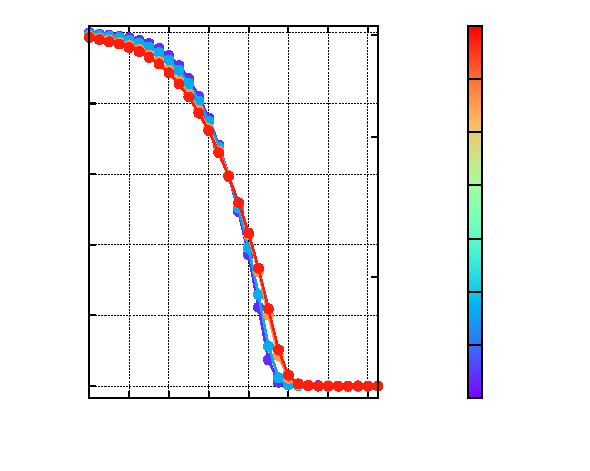
\includegraphics{LudoxHS40TransmissionCalibration}}%
    \gplfronttext
  \end{picture}%
\endgroup

		\caption[Concentration gradient of 12 nm silica particles measured at 8000 eV.]{Concentration gradient of 12 nm silica particles measured at 8000 eV. The large size of the colloids in comparison to a saccharide molecule provides a longer diffusion time than a typical contrast agent like sucrose.}
		\label{fig:LudoxHS40TransmissionCalibration}
\end{figure*}

In figure \ref{fig:LudoxHS40TransmissionCalibration}, the calibrated transmittance of a density gradient capillary of aqueous 12 nm silica nanoparticles (Ludox HS40, Sigma-Aldrich, Missouri, USA) is depicted, where the particle concentration is a function of the capillary height. The slower evolution of the concentration gradient compared with sucrose in figure \ref{fig:KiskerTransmissionCalibration} and the large density difference between water and the high concentrated particle suspension (ca. 1.3 g cm$^{-3}$) can improve the quality of the X-ray transmission data and provide an alternative application of the \emph{density gradient} technique in SAXS, where the diffusive agent is the investigated object. Moreover, table-top X-ray sources can be an alternative to high photon flux synchrotron radiation sources due to the extended experimental timescale achieved when using colloids as diffusing agent.

A colloidal concentration gradient as presented in figure \ref{fig:LudoxHS40TransmissionCalibration} can be used to study the effects of concentration on the diffusion constant of the particles or investigate the type of inter-particle interactions as a function of the colloidal concentration. For example, standard dilution series can be performed \emph{in situ} with this approach or examine the crystallization of the particles under gravitational forces \citep{hellsing_structure_2012}. 
